\chapter{Results and discussion}

\section{Avinor lightning data set}\label{sec:avinor}

\begin{figure}
    \centering
    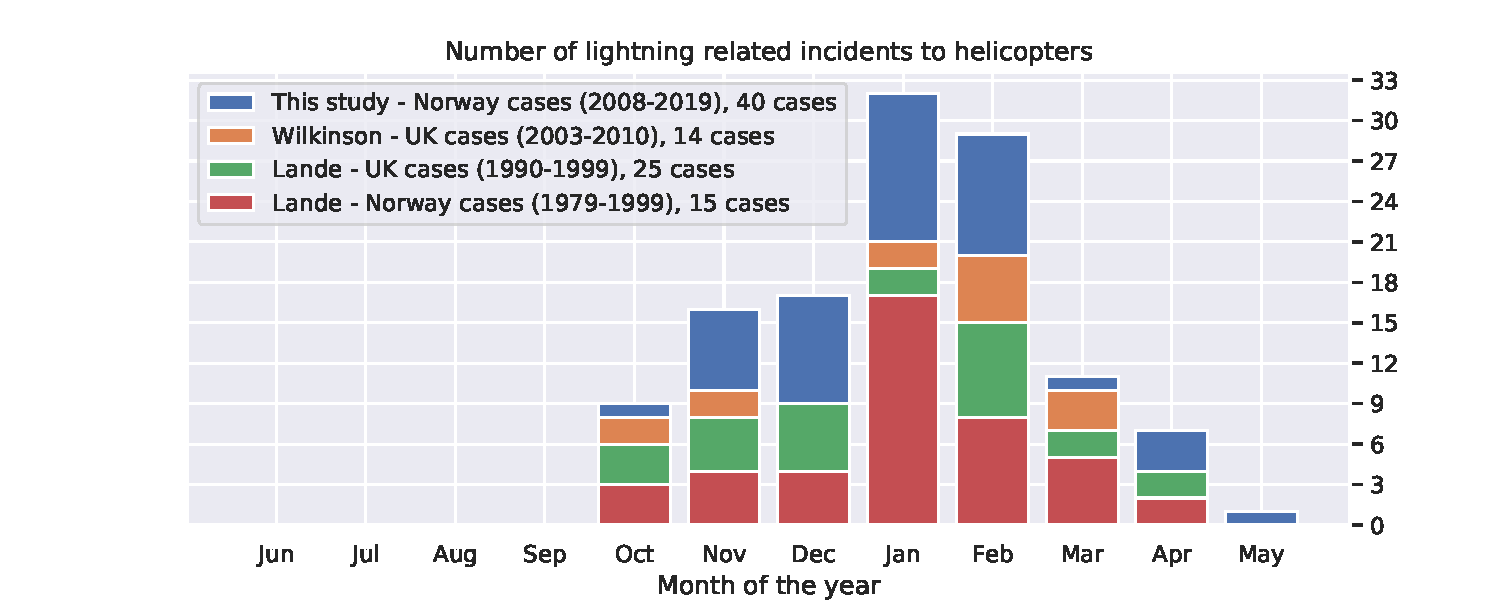
\includegraphics[width=\textwidth]{Figures/yearlydistribution.pdf}
    \caption{Seasonal variation of helicopter cases, showing no cases in June to September. Same as Figure \ref{fig:landewilk}, with cases looked at in this study added to it. Older data is produced from \cite{lande1999} and \cite{wilkinson2013}. Legend notes time-periods and amount of cases in each study. }
    \label{fig:yearlyvariation}
\end{figure}

\begin{figure}
    \centering
    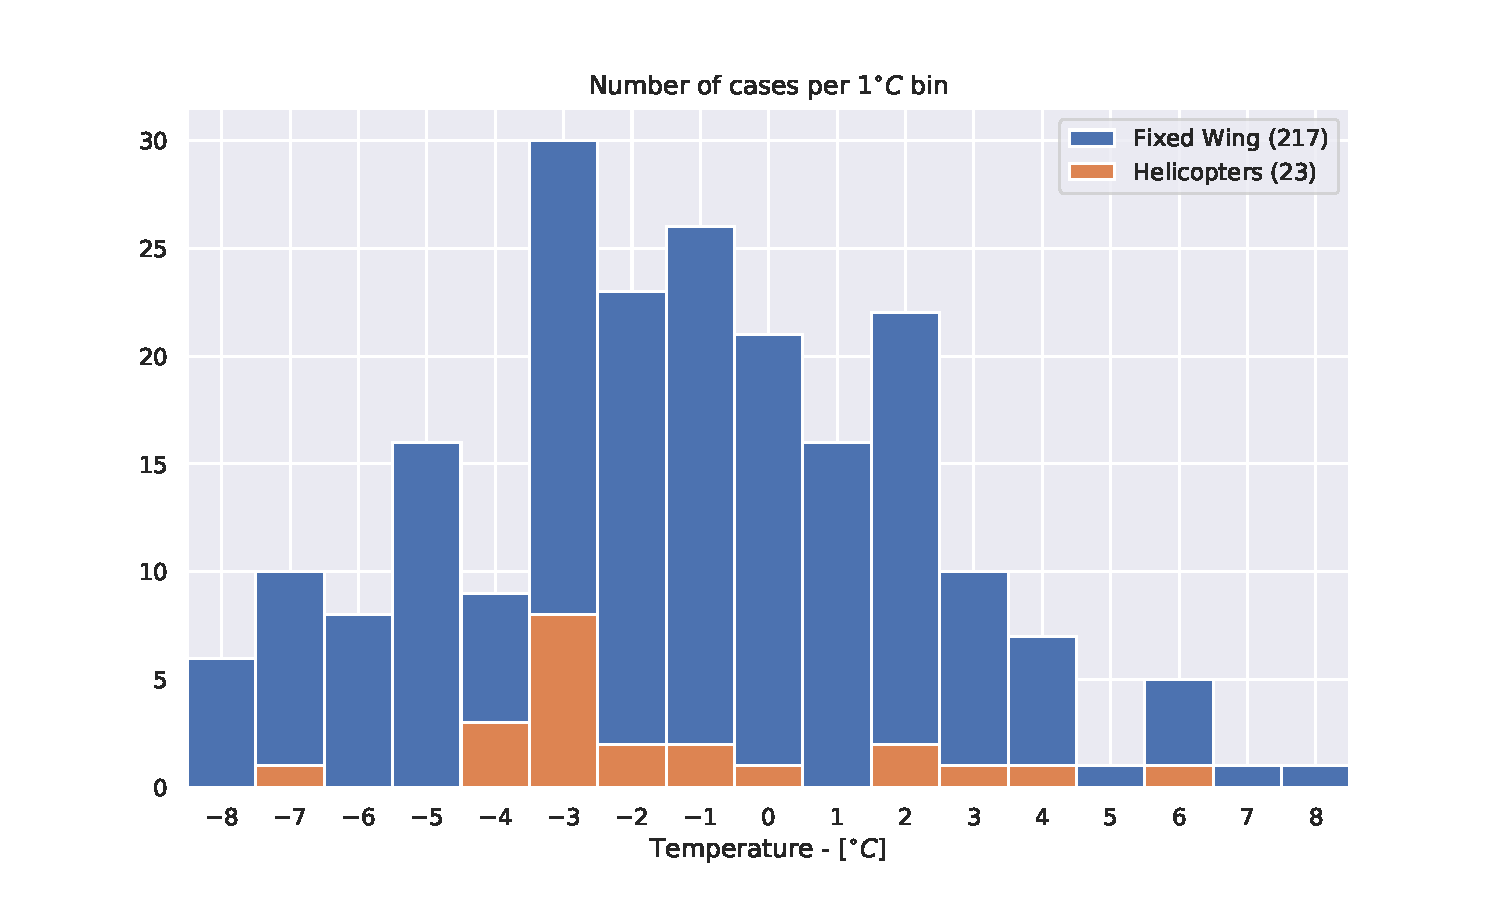
\includegraphics[width=\textwidth]{Figures/temperature.pdf}
    \caption{Temperature in fixed-wing and helicopter cases (interpolated from ERA5 pressure levels)}
    \label{fig:temperatureera5}
\end{figure}

As discussed in Chapter \ref{ch:lightning}, there exists a body of research showing that the $0^{\circ}C$ isotherm in a cloud is related to winter- and \acrlong{htl}. Figure \ref{fig:yearlyvariation} shows that the Avinor data set has the same seasonal variation as these earlier studies, except for the additional case in May. This is presumably due to the Norwegian climate being generally colder than the British, which is where most of the earlier cases were from. 

In contrast to the earlier research, the temperature found from ERA5 in Figure \ref{fig:temperatureera5} shows that the peak is situated around $-3^{\circ}C$ and not the $0^{\circ}C$ isotherm. This can either be attributed to a systematic error in pressure level interpolation (see Section \ref{sec:interpolation}), or due to operational procedures implemented due to \cite{lande1999}, which advises avoidance of the $0^{\circ}C$ isotherm when \acrshort{htl} is forecast or when flying inside of a cloud. Taking into account the \acrshort{fwtl} temperature in the same figure, there seems to be a $-1^{\circ}C$ shift from $0^{\circ}C$ since the peaks are at $-1^{\circ}C$ and $-3^{\circ}C$ compared to Figure \ref{fig:landetemp}. This also supports the previous statement about the effect of avoiding the $0^{\circ}C$ isotherm, as this is not a procedure followed by pilots flying fixed wing aircraft.

Figure \ref{fig:helisoner} shows the \acrshort{htl} incidents divided by the zones shown in Figure \ref{fig:Stationsmap}. It should be noted that there are no cases at Gardermoen, and only one case off the coast of Denmark in the Southern coast zone. The April peak is primarily contributed to by the North coast zone, which can be explained by the fact that the sea is still relatively warmer than the atmosphere during this time compared to the coast further south. This therefore supports earlier work in which it was proposed that cold air over warmer oceans caused convective systems to appear and be electrified. 

Figure \ref{fig:helivsfw} shows the same picture that \acrshort{htl} is a winter phenomenon and supports the claim in Section \ref{sec:fwtl} that \acrshort{fwtl} is an all-year phenomenon. The august peak in \acrshort{fwtl} can be explained by August being the month with the highest lightning activity in Norway. July also has some lightning activity, but commercial air travel is reduced compared to August. 

Figure \ref{fig:soner} shows that there is a geographical variation in cases, namely southern coast and Gardermoen primarily have cases during April-October, whereas the north, west and northwest are more represented during October-April. This shows a similar picture to that in \cite{koeltzow2018}: The Norwegian lightning climatology is primarily coastal in nature for winter lightning, and primarily inland for summer lightning. 

\begin{figure}
    \centering
    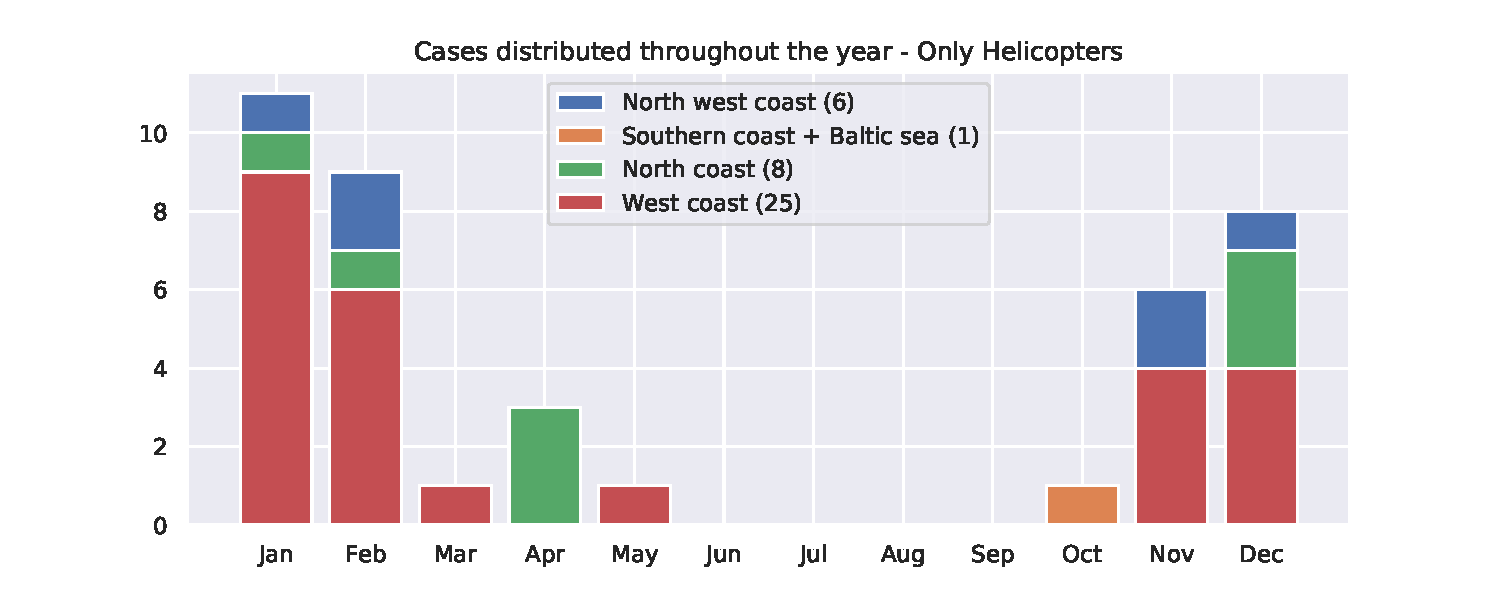
\includegraphics[width=\textwidth]{Figures/Helisoner.pdf}
    \caption{Zonal division of helicopter cases}
    \label{fig:helisoner}
\end{figure}

\begin{figure}
    \begin{subfigure}{\textwidth}
    \centering
    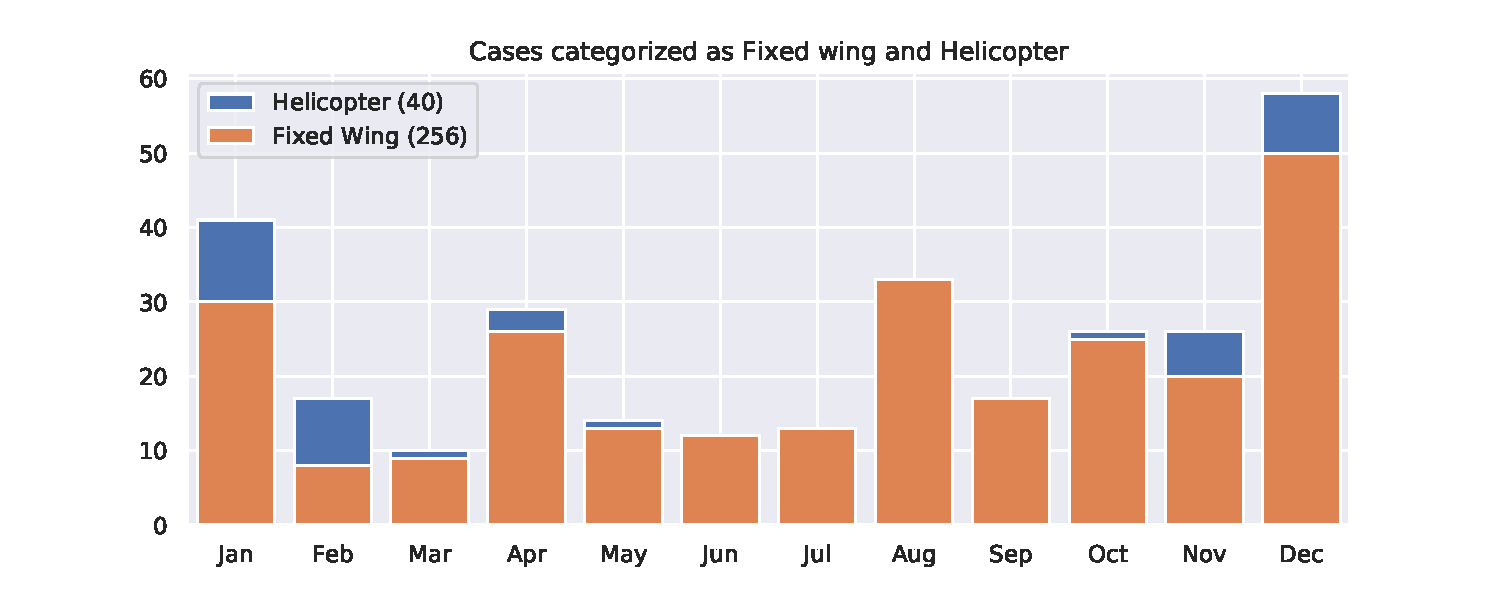
\includegraphics[width=\textwidth]{Figures/helivsfw.pdf}
    \caption{Yearly distribution of helicopter and fixed wing cases}
    \label{fig:helivsfw}
    \end{subfigure}
    
    \begin{subfigure}{\textwidth}
    \centering
    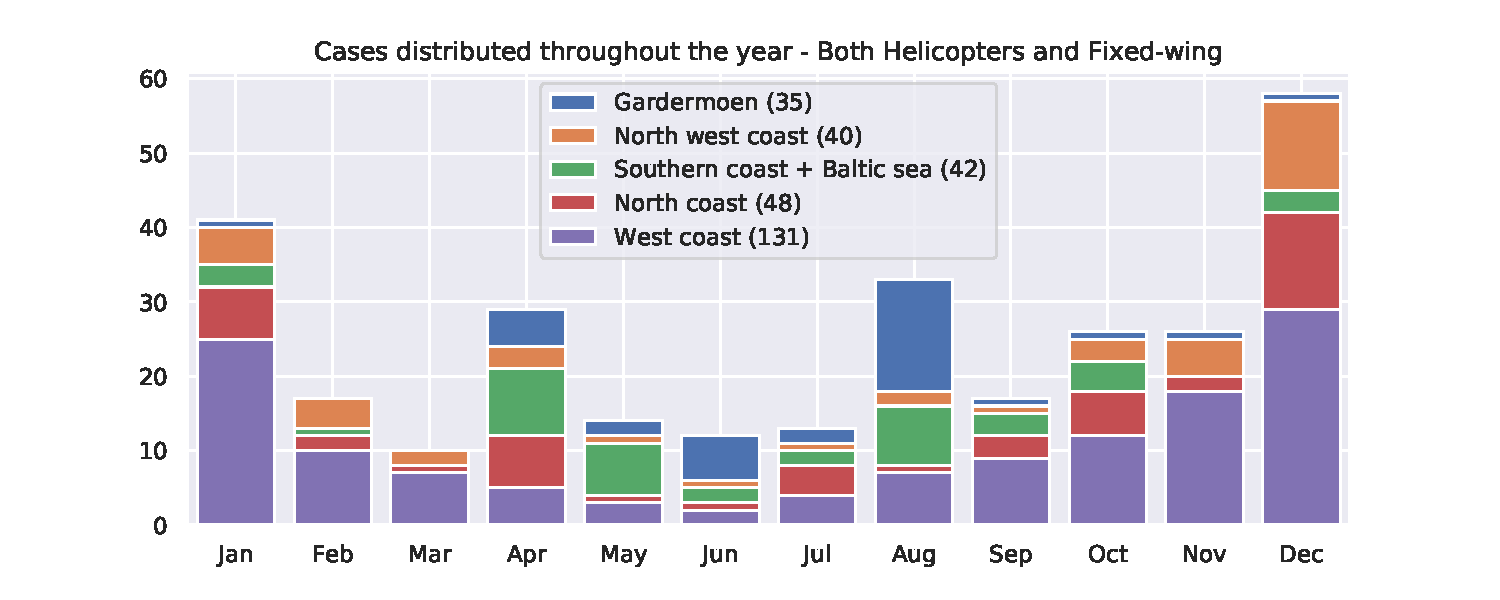
\includegraphics[width=\textwidth]{Figures/soner.pdf}
    \caption{Zonal division of helicopter and fixed wing cases, see Figure \ref{fig:helivsfw} for categorical distribution}
    \label{fig:soner}
    \end{subfigure}
\end{figure}

\section{What meteorological phenomena are observed during a triggered lightning incident?}

Figure \ref{fig:metarcases} shows the meteorological phenomena reported in the METAR report during triggered lightning incidents (both \acrshort{htl} and \acrshort{fwtl}). The helicopter cases show a high frequency (above 50 $\%$) for scattered, few and broken clouds, but zero of the cases had overcast conditions. Also found were showers in 20 $\%$ of the cases, and rain and/or snow was found in more than 20 $\%$ of the cases. Only 20 $\%$ of the cases had a report of cumulonimbus clouds. For the fixed wing, the cumulonimbus frequency is much higher (60 $\%$), and rain was in 40 $\%$ of the cases and snow in less than 5 $\%$. Showers were also often reported (60 $\%$). The fact that snow was less often reported for fixed wing compared to helicopter cases may be due to it being an all-year phenomenon such that snow was not observed at the ground during summer events. This, in turn, supports both \cite{lande1999} in that cumulonimbus was not \textit{always} observed during triggered lightning incidents, and the choice to include maximum cloud cover minus minimum cloud cover since almost none of the cases show overcast conditions.

\begin{figure}
    \centering
    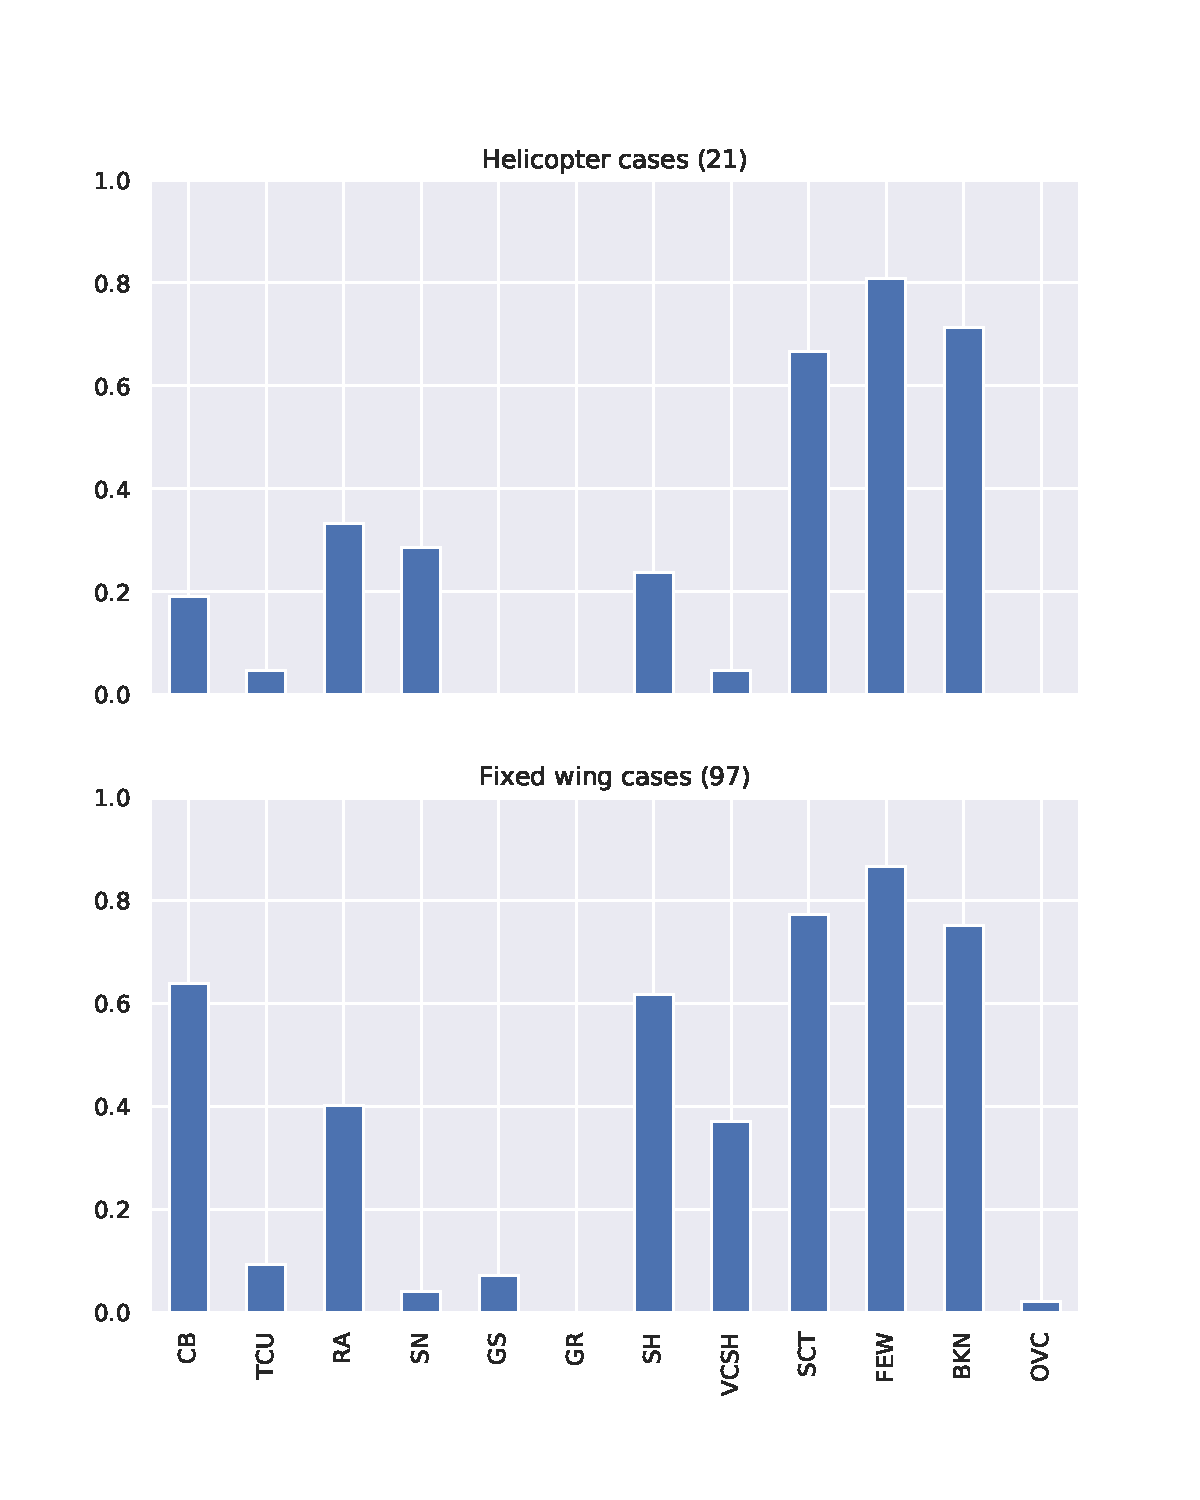
\includegraphics[width=\textwidth]{Figures/METARcases.pdf}
    \caption{Frequency of different categories of METAR-phenomenon for Helicopter and Fixed wing cases, included are only cases where airport had a METAR-report that was taken by a non-automatic system. Note that SH also include VCSH}
    \label{fig:metarcases}
\end{figure}

\begin{figure}
    \centering
    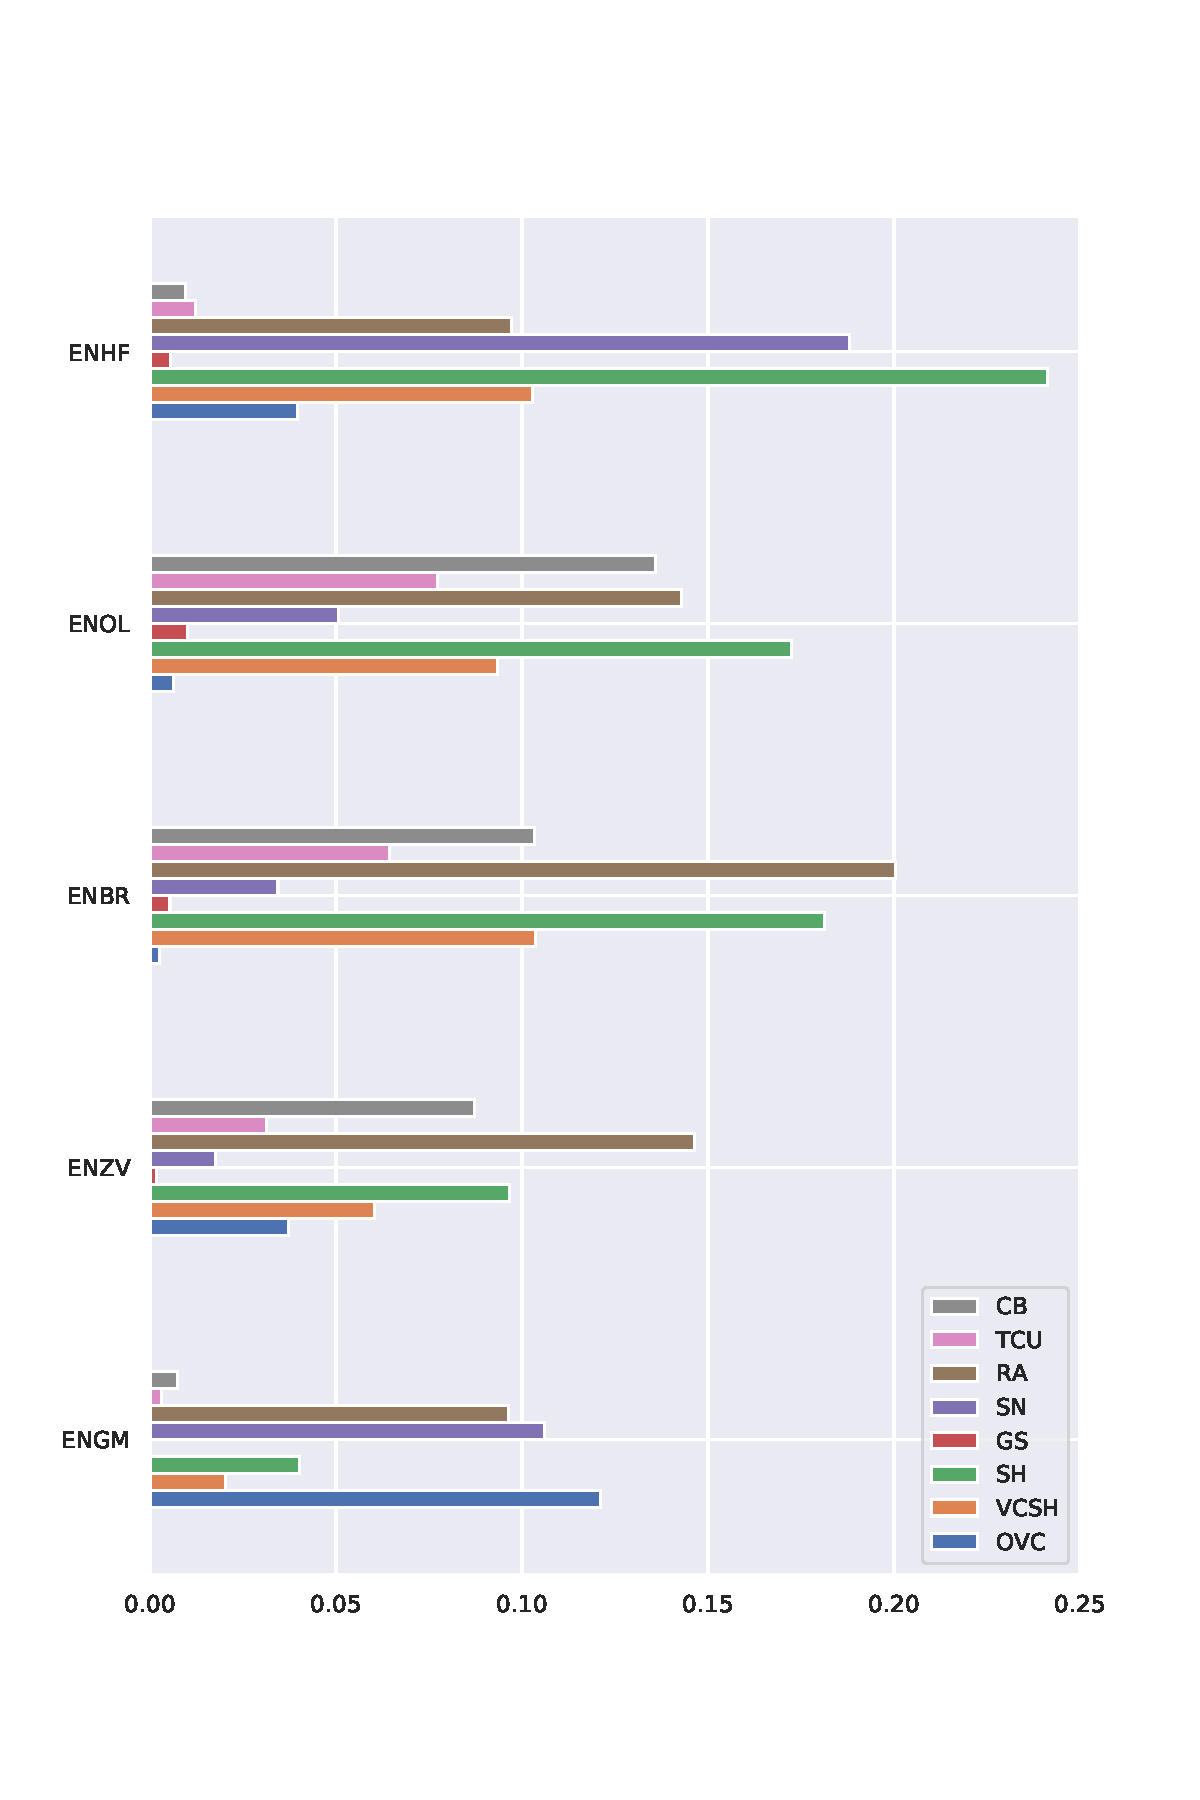
\includegraphics[width=.9\textwidth]{Figures/METAR_airports.pdf}
    \caption{Percentage of METAR-reports involving at least one of the meteorological phenomena at Hammerfest, Ørlandet, Flesland, Sola, and Gardermoen airports. Selection is based on geographical variation and representation.}
    \label{fig:metarclimat}
\end{figure}


\subsection{Why are there more HTL near Flesland than Sola?}

Looking at the flight traffic data compared to triggered lightning events in Table \ref{tab:traffic}, it is clear that Flesland airport has the highest incident per traffic ratio of the large Norwegian airports. 

Figure \ref{fig:metarclimat} shows Flesland to have a higher (20$\%$) frequency of rain than Sola at 15$\%$. The same is seen for both categories of showers (\textit{SH}, \textit{VCSH}). This suggests a more convective area around Flesland airport than at Sola airport. Ørlandet has similar convective activity to Flesland, but has almost no commercial air traffic. Therefore, any triggered lightning incident would not be in this data set and there is a smaller amount of potential trigger events. 

This convective difference between Flesland and Stavanger cannot be explained by yearly traffic differences, and their geographical positions are so close that there should not be any substantial climatological temperature differences between the two. There is somewhat less lightning activity observed at Flesland compared to Sola.

\begin{table}
        \begin{tabular}{r|l|l|l|}
            & Sola (ENZV) & Flesland (ENBR) & Gardermoen (ENGM) \\\hline
            Average yearly traffic (2016-2018)  & 74 532 & 92 128 & 253 599   \\\hline
            Lightning close to airport (2008-2019) & 30 920 & 22 774 & 68 321 \\\hline
            Cases close to airport & 24 & 63  & 35 \\\hline
            Case per traffic  & 1 / 31 055 & 1 / 14 624 & 1 / 72 457 \\\hline
            Case per recorded lightning & 1 / 1 289 & 1 / 361 & 1 / 1 952 \\\hline
        \end{tabular}
     \caption{Average traffic, accumulated lightning activity, and cases within $0.5^{\circ}$($\approx 50km$) radius of the three biggest Norwegian airports.}
     \label{tab:traffic}
\end{table}



\section{What are the composites telling us about the atmospheric conditions during triggered lightning incidents?}\label{sec:compositesera5}
To investigate the parameters used in the operational \acrshort{hti} forecast, composites have been created for the cases from the Avinor data set. The parameters studied are temperature, vertical velocity, precipitation and cloud cover. Cloud cover did not show any clear signal due to ERA5 horizontal scale, and therefore was moved to Appendix \ref{app:A}. Also studied is the general circulation during these cases, by looking at the composite of the mean sea level pressure. 

\subsection{Temperature during triggered lightning events}
Shown in Figure \ref{fig:tempzones} are temperature composites divided into the geographical zones described in Appendix \ref{app:B}. The figure reveals that for the different geographic zones, the average temperature in the composites are around -3 to 0$^{\circ}C$. This is in accordance with previous findings that \acrshort{htl} happens at temperatures right below or at 0$^{\circ}C$. One also sees that grouping of the cases leads to a reduction in the standard deviation along each zone's coast, except for the North zone. This hints to that these temperatures are closely related, but North zone should ideally be divided into finer zones. (This would, however, be less robust due to the North zone only containing 40 cases.)

Figure \ref{fig:tempairports} shows that the temperatures at Flesland and Sola are, as expected, around 0 to -1$^{\circ}C$, and here the variation in temperature is much lower as seen in the respective standard deviation plots. The standard deviation is lowest in Flesland, but this is to be expected, since there are double the amount of cases at Flesland than Sola. Looking, though, at Figure \ref{fig:ENGMTemperature}, one sees that Gardermoen airport has a much warmer situation at around +2$^{\circ}C$. Here, the standard deviation also is higher. This coincides with the variation shown in Figure \ref{fig:temperatureera5}. 

\subsection{Typical pressure pattern during triggered lightning events}
Figure \ref{fig:tempzones} contains, in addition to temperature, composites of pressure during triggered lightning events. The general circulation from these pressure systems seems to tend toward geostrophic wind directed toward the coast. Notable exception is the South zone, which does not have a clear low pressure system in the ocean, but the standard deviation hints to a lot of variation over the ocean. The geostrophic winds for the remaining zones also would be coming from colder areas, i.e. Iceland and the Arctic. This would lead to cold air being blown over the relatively warm North Atlantic Current, as discussed in Section \ref{sec:winter lightning}, as a precursor for convection and lightning activity. The pressure in Figure \ref{fig:tempairports} shows the same picture for both Flesland and Sola airports, being dominated by low pressure systems situated in the Norwegian Sea, such that the geostrophic wind would be directed inland toward the airports. The convection may be a result of topography and surface roughness changing when moving from ocean to land. Since the land does not dissipate the energy in form of waves, the energy leads to more turbulence in the air, causing local convection. This suggests that wind incident on land is present in most cases of triggered lightning events at the coast of Norway. 

However, Gardermoen being located inland does not see this roughness effect. This suggests that incidents at Gardermoen are instead related to local convective systems seen in the summertime. This explains why Gardermoen airport's pressure situation is "normal" during triggered lightning events, since the incidents are related to local convective systems rather than bigger circulation causing local convection. The standard deviation shows the same picture in that the pressure does not have a large standard deviation.

\begin{figure}
\begin{subfigure}[b]{0.49\textwidth}
    \centering
    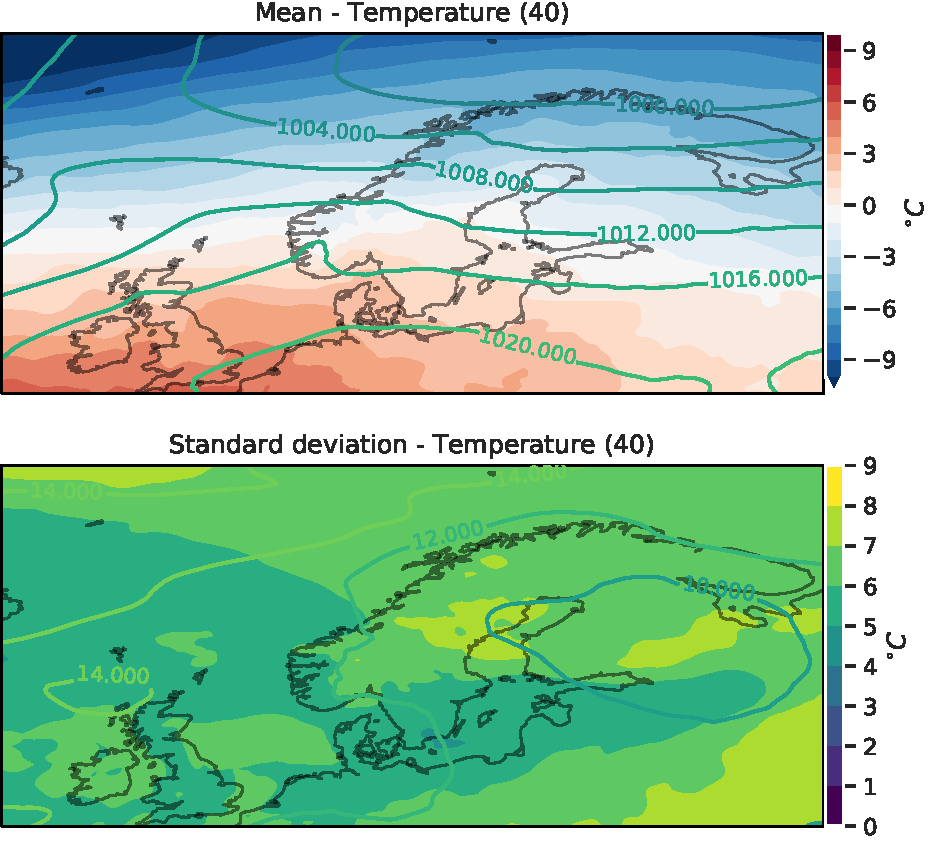
\includegraphics[width=\textwidth]{Figures/TempNord.pdf}
    \caption{Temperature for cases in North zone.}
    \label{fig:NordTemperature}
\end{subfigure}
\begin{subfigure}[b]{0.49\textwidth}
    \centering
    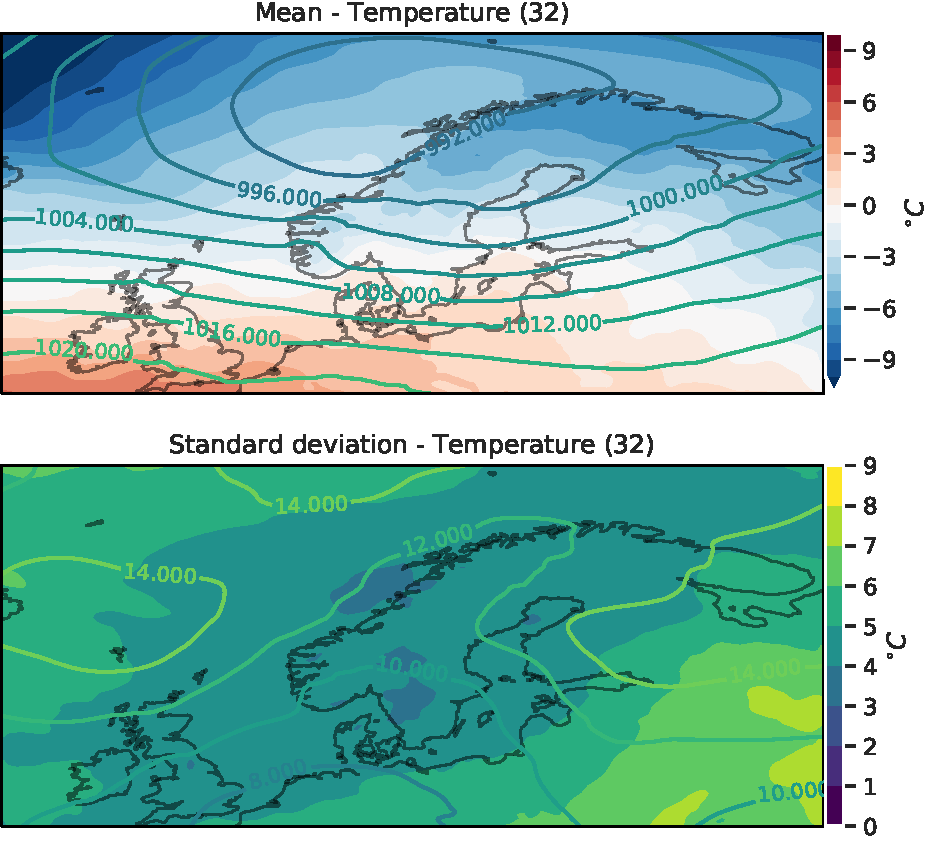
\includegraphics[width=\textwidth]{Figures/TempNordvest.pdf}
    \caption{Temperature for cases in Northwest zone.}
    \label{fig:NordWestTemperature}
\end{subfigure}
\begin{subfigure}[b]{0.49\textwidth}
    \centering
    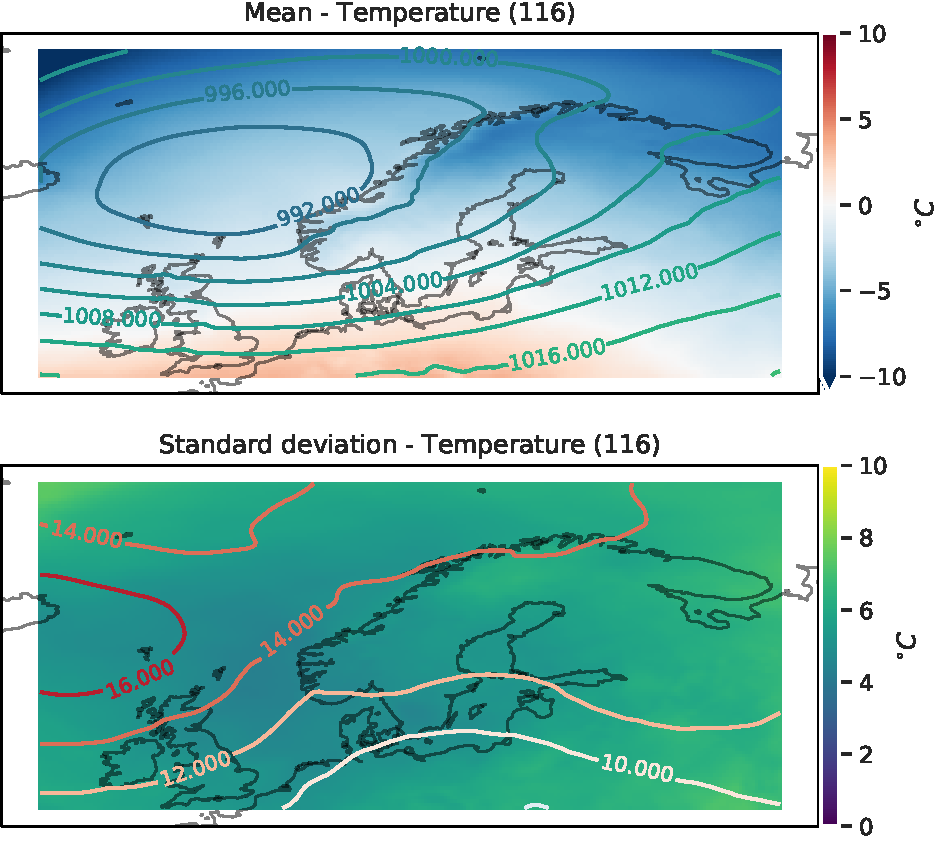
\includegraphics[width=\textwidth]{Figures/TempVest.pdf}
    \caption{Temperature for cases in West zone.}
    \label{fig:WestTemperature}
\end{subfigure}
\begin{subfigure}[b]{0.49\textwidth}
    \centering
    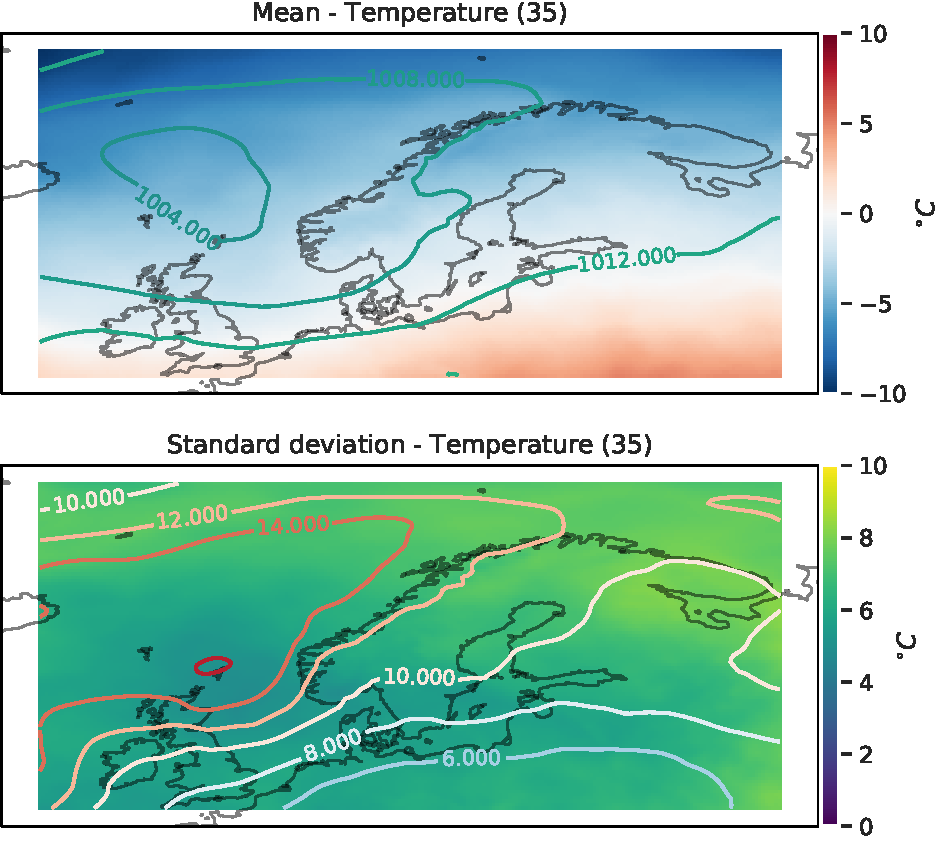
\includegraphics[width=\textwidth]{Figures/TempSor.pdf}
    \caption{Temperature for cases in South zone.}
    \label{fig:SouthTemperature}
\end{subfigure}
\caption{Temperature composites for both \acrshort{htl} and \acrshort{fwtl} cases in different geographical zones. Included are only cases for which height information was provided in the Avinor data set. The temperature was found by interpolating to the correct height as described in Section \ref{sec:interpolation}}
\label{fig:tempzones}
\end{figure}

\begin{figure}
     \centering
     \begin{subfigure}[b]{0.49\textwidth}
         \centering
         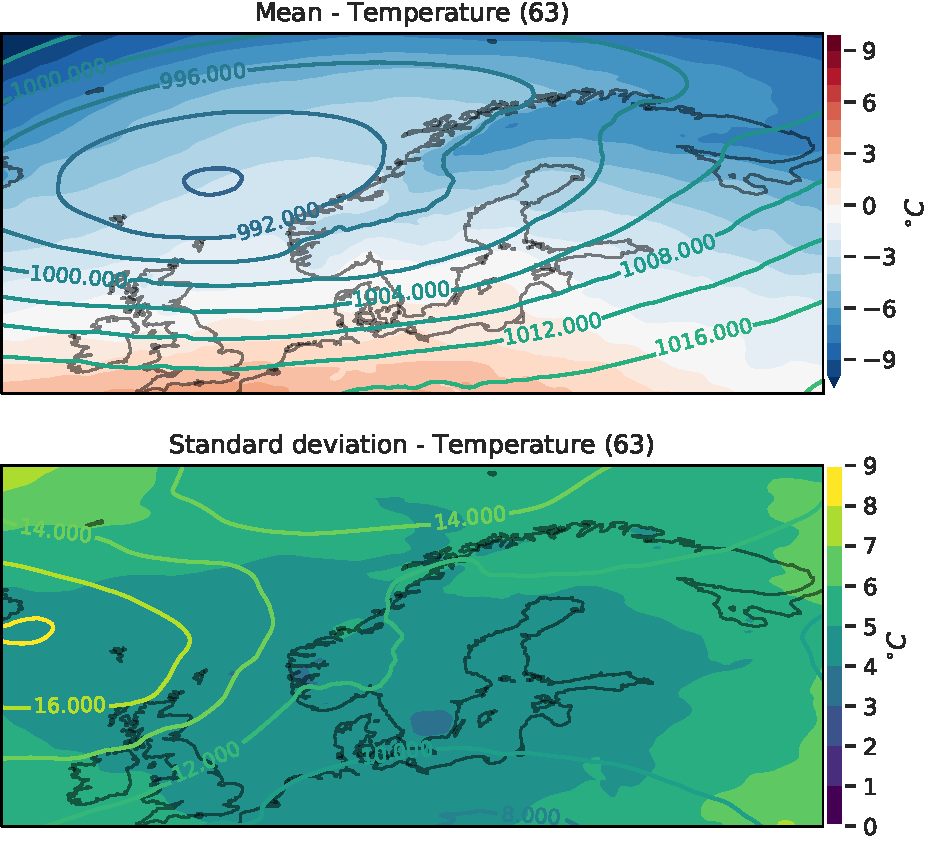
\includegraphics[width=\textwidth]{Figures/TempENBR.pdf}
         \caption{Temperature for cases at Flesland airport.}
         \label{fig:ENBRTemperature}
     \end{subfigure}
     \hfill
     \begin{subfigure}[b]{0.49\textwidth}
         \centering
         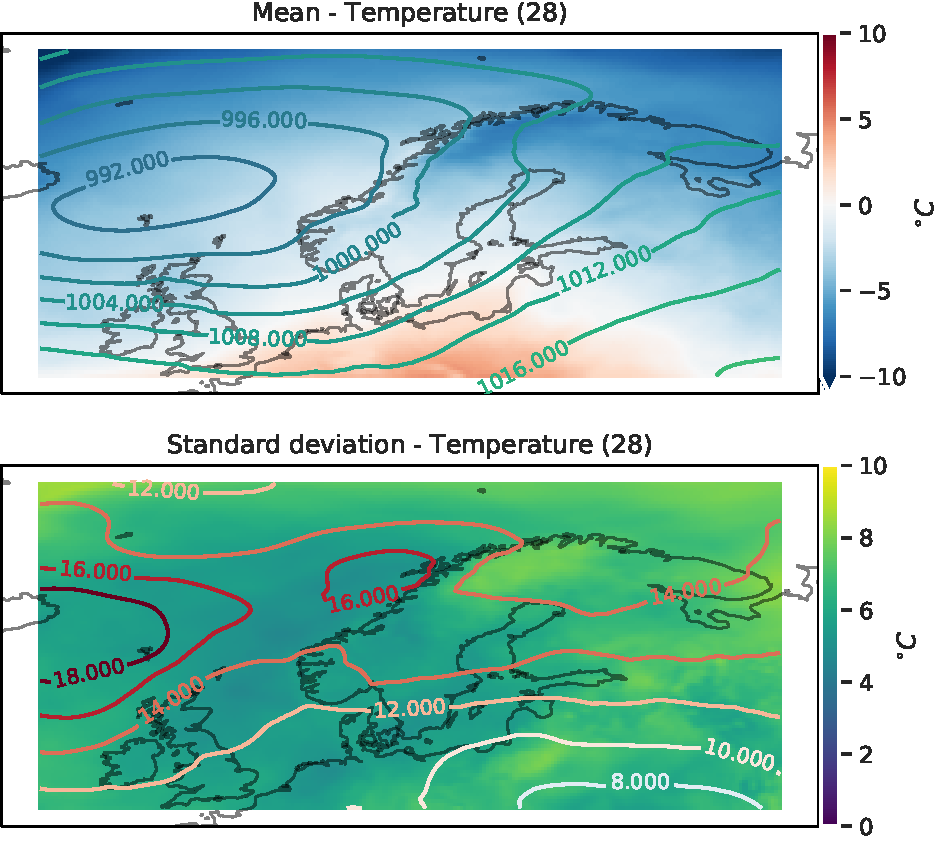
\includegraphics[width=\textwidth]{Figures/TempENZV.pdf}
         \caption{Temperature for cases at Sola airport.}
         \label{fig:ENZVTemperature}
     \end{subfigure}

    \begin{subfigure}[b]{0.5\textwidth}
    \centering
    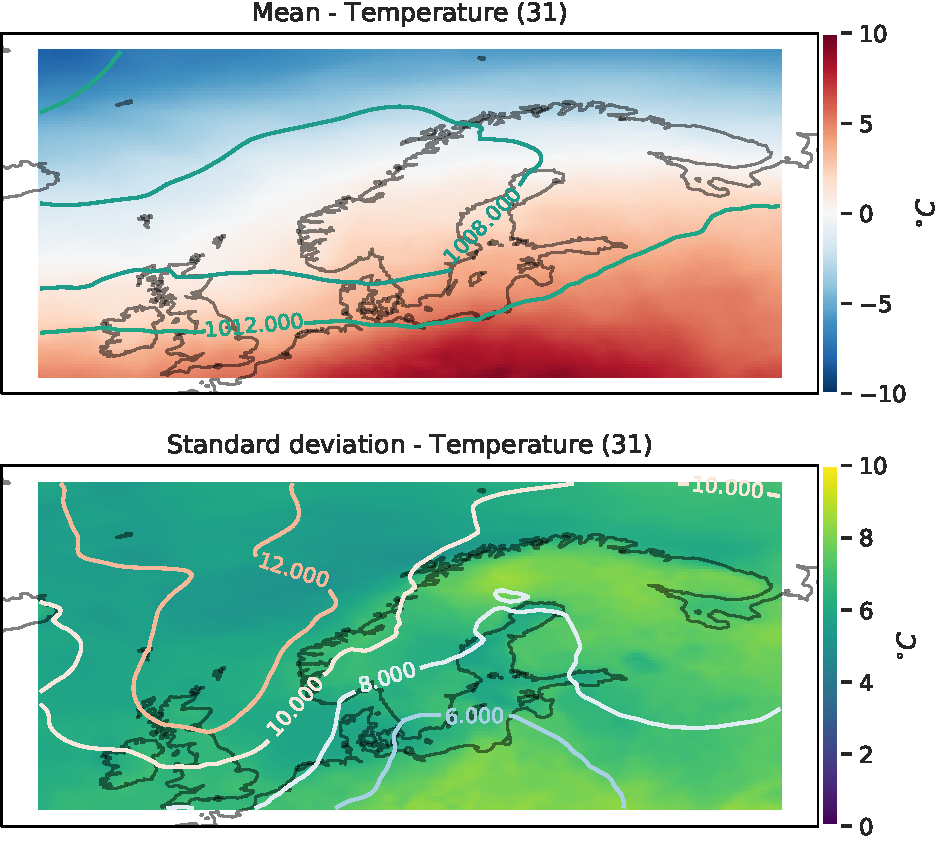
\includegraphics[width=\textwidth]{Figures/TempENGM.pdf}
    \caption{Temperature for cases in Gardermoen zone.}
    \label{fig:ENGMTemperature}
\end{subfigure}
\caption{Same as Figure \ref{fig:tempzones}, but for only the biggest airports. }
\label{fig:tempairports}
\end{figure}

\subsection{Vertical velocity during triggered lightning events}\label{sec:verticalvelocity}

Figure \ref{fig:verticalzones} shows vertical velocity composites for the different geographic zones. It should be noted that the color bar is inverted, such that red is negative and blue is positive. This is done due to the units being Pa/s, so that negative values infers upward velocity and positive downward velocity. One can see a clear trend among the coastal zones (north, northwest and west) that there is upward vertical velocity related to the cases. There is also a somewhat high standard deviation in these same zones, but this could be related to \textit{placing} of the upward velocity systems in the model. Looking at Figure \ref{fig:verticalairports}, one sees the same for both Flesland and Sola: A clear vertical velocity in the composite, but some higher standard deviation in the Sola case. (Again, presumably because of the lower number of cases.) There is a very weak vertical velocity for the Gardermoen case. This can be explained by Gardermoen predominantly being subject to summer lightning, which is due to local convective areas and may not be correctly resolved in the coarse horizontal grid of ERA5. 

\begin{figure}
\begin{subfigure}[b]{0.49\textwidth}
    \centering
    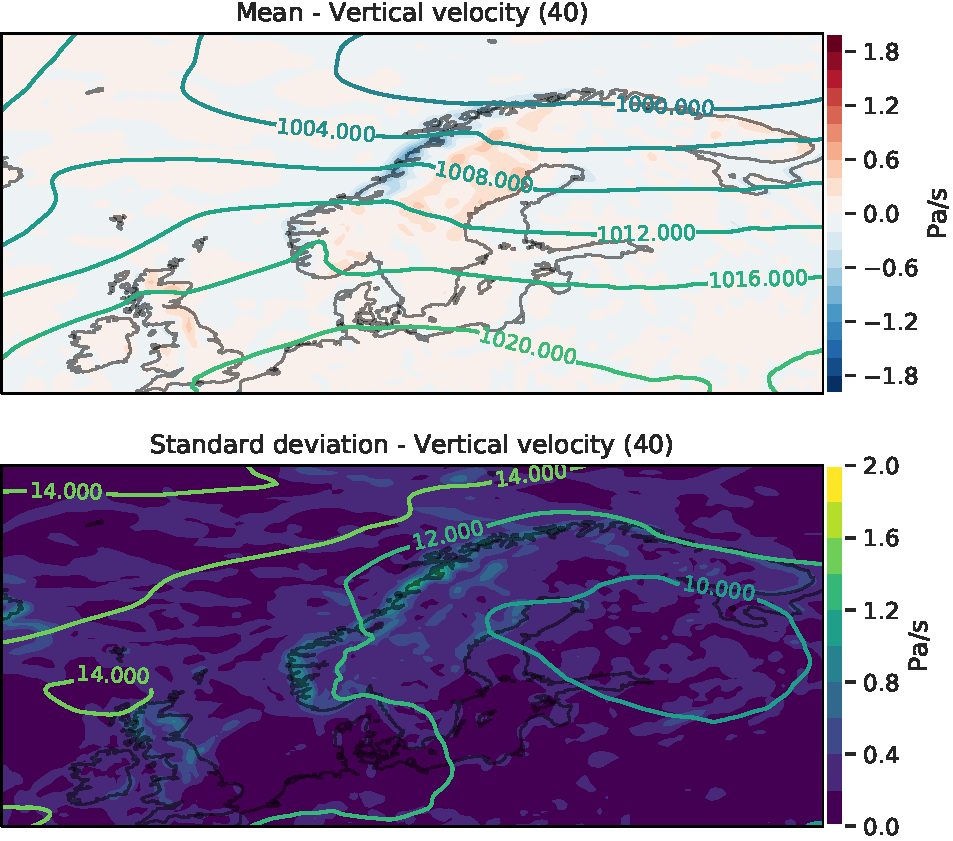
\includegraphics[width=\textwidth]{Figures/WNord.pdf}
    \caption{Vertical velocity for cases in North zone.}
    \label{fig:NordW}
\end{subfigure}
\begin{subfigure}[b]{0.49\textwidth}
    \centering
    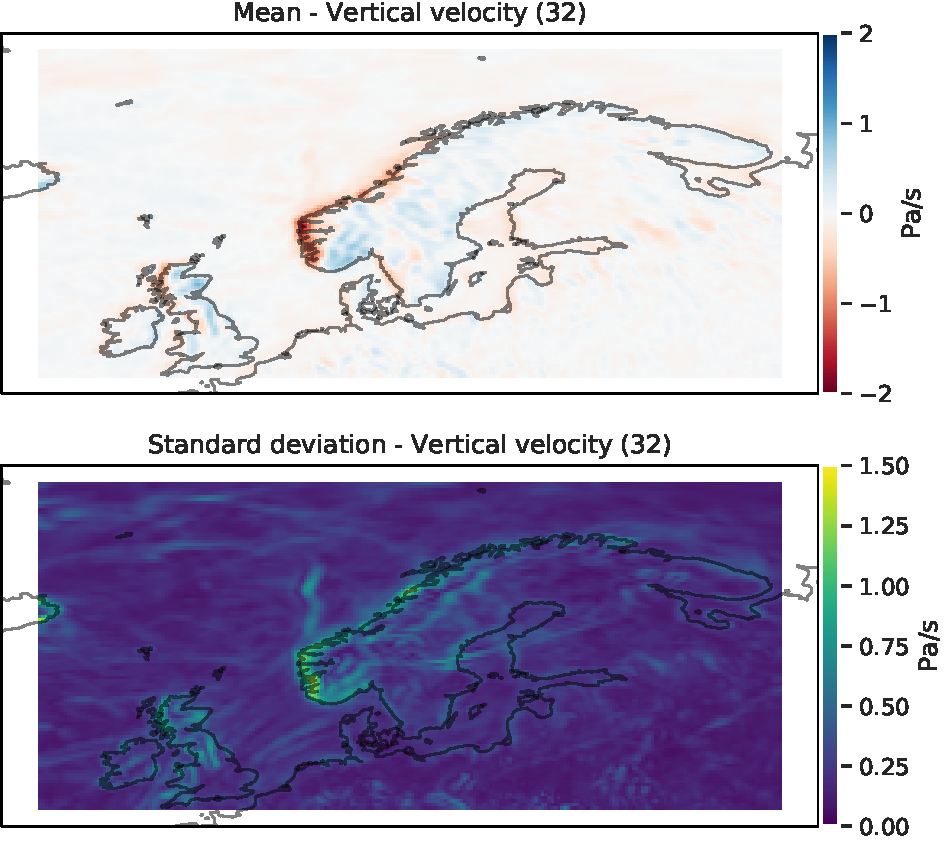
\includegraphics[width=\textwidth]{Figures/WNordvest.pdf}
    \caption{Vertical velocity  for cases in Northwest zone.}
    \label{fig:NordWestW}
\end{subfigure}
\begin{subfigure}[b]{0.49\textwidth}
    \centering
    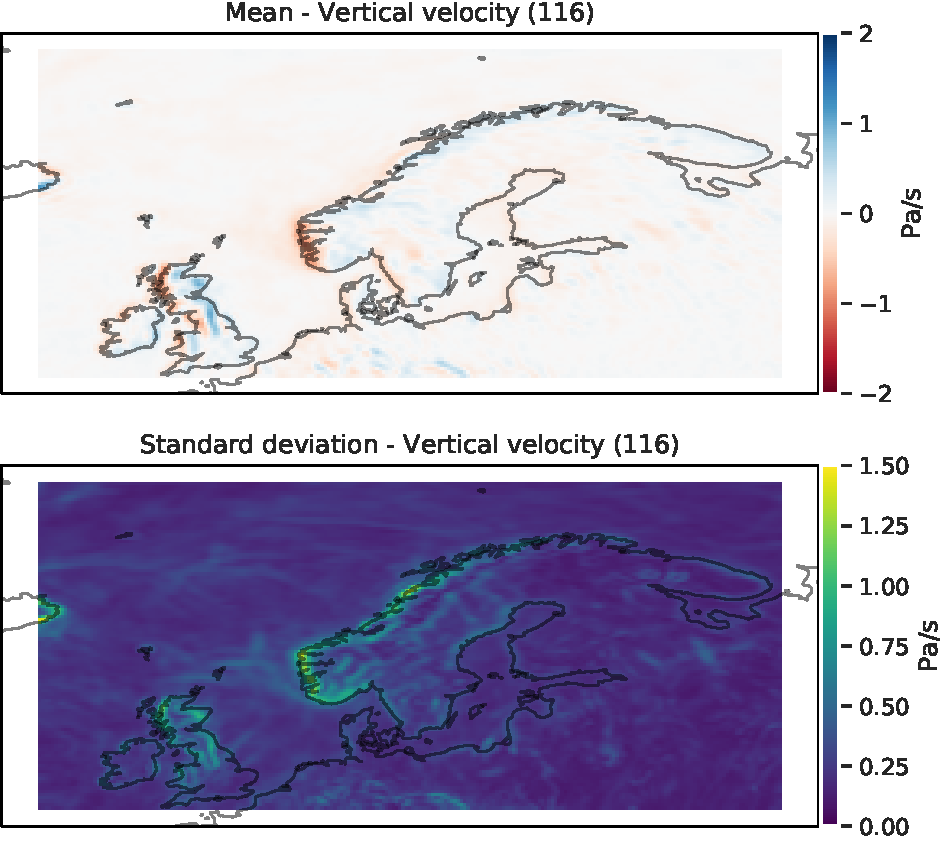
\includegraphics[width=\textwidth]{Figures/WVest.pdf}
    \caption{Vertical velocity  for cases in West zone.}
    \label{fig:WestW}
\end{subfigure}
\begin{subfigure}[b]{0.49\textwidth}
    \centering
    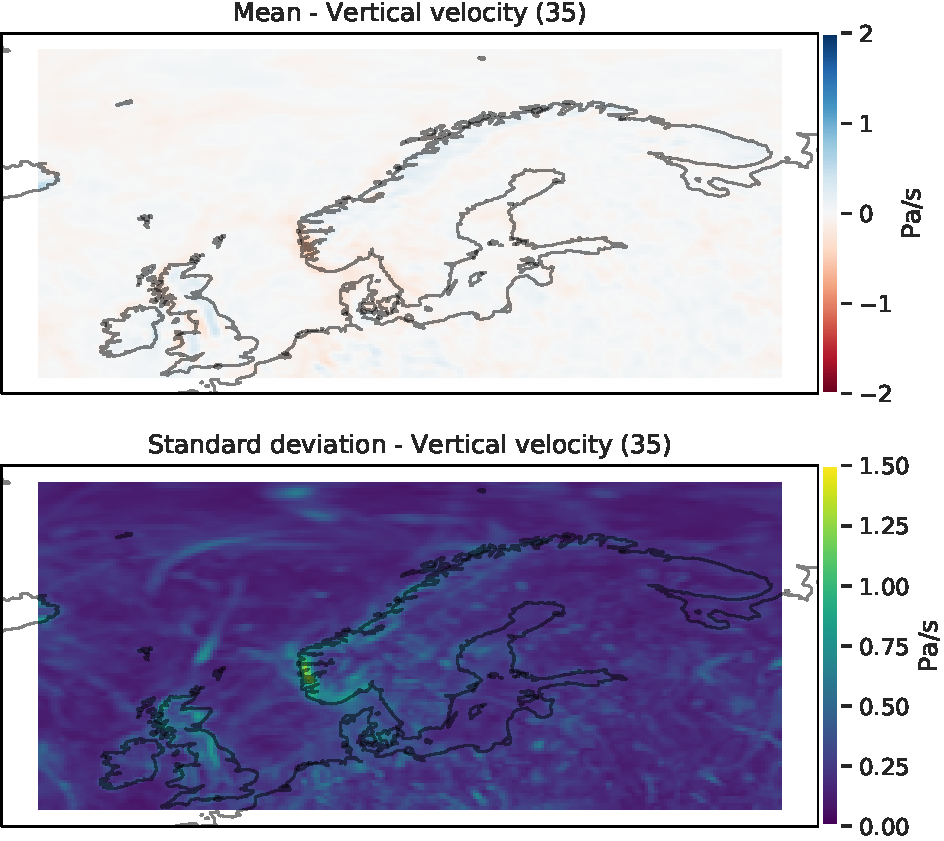
\includegraphics[width=\textwidth]{Figures/WSor.pdf}
    \caption{Vertical velocity  for cases in South zone.}
    \label{fig:SouthW}
\end{subfigure}
\caption{Vertical velocity composites for both \acrshort{htl} and \acrshort{fwtl} cases in different geographical zones. Included are only cases for which height information was provided in the Avinor data set. The velocity was found by interpolating to the correct height as described in Section \ref{sec:interpolation}}
\label{fig:verticalzones}
\end{figure}

\begin{figure}
     \centering
     \begin{subfigure}[b]{0.49\textwidth}
         \centering
         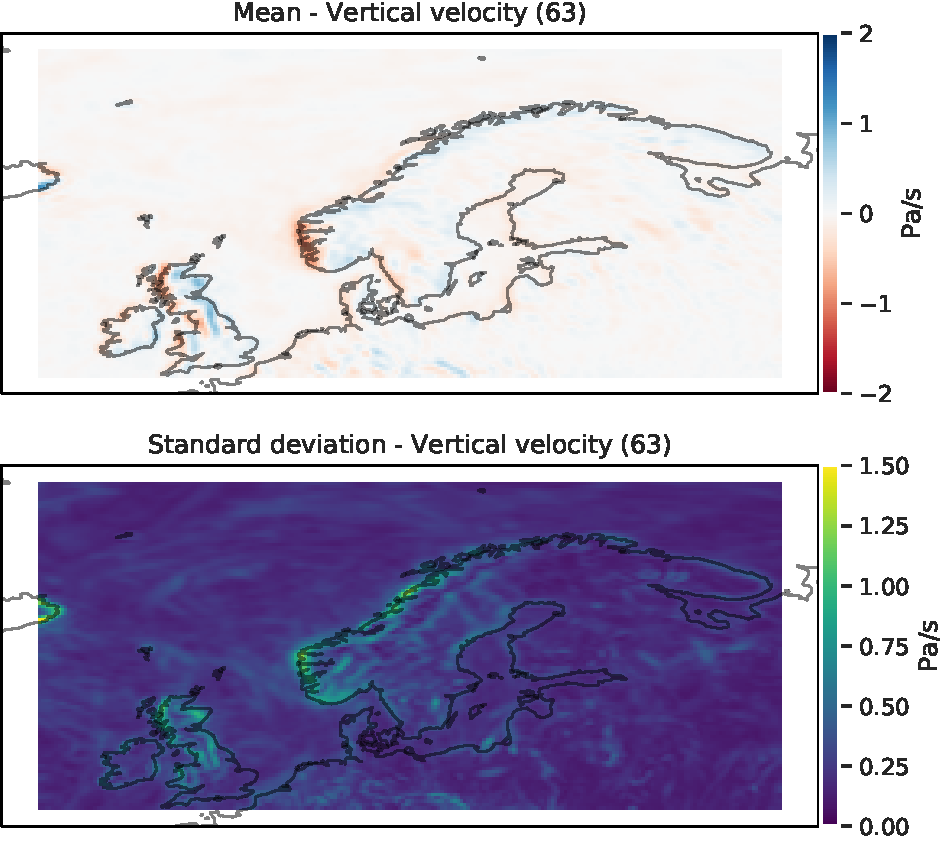
\includegraphics[width=\textwidth]{Figures/WENBR.pdf}
         \caption{Vertical velocity for cases at Flesland}
         \label{fig:ENBRW}
     \end{subfigure}
     \hfill
     \begin{subfigure}[b]{0.49\textwidth}
         \centering
         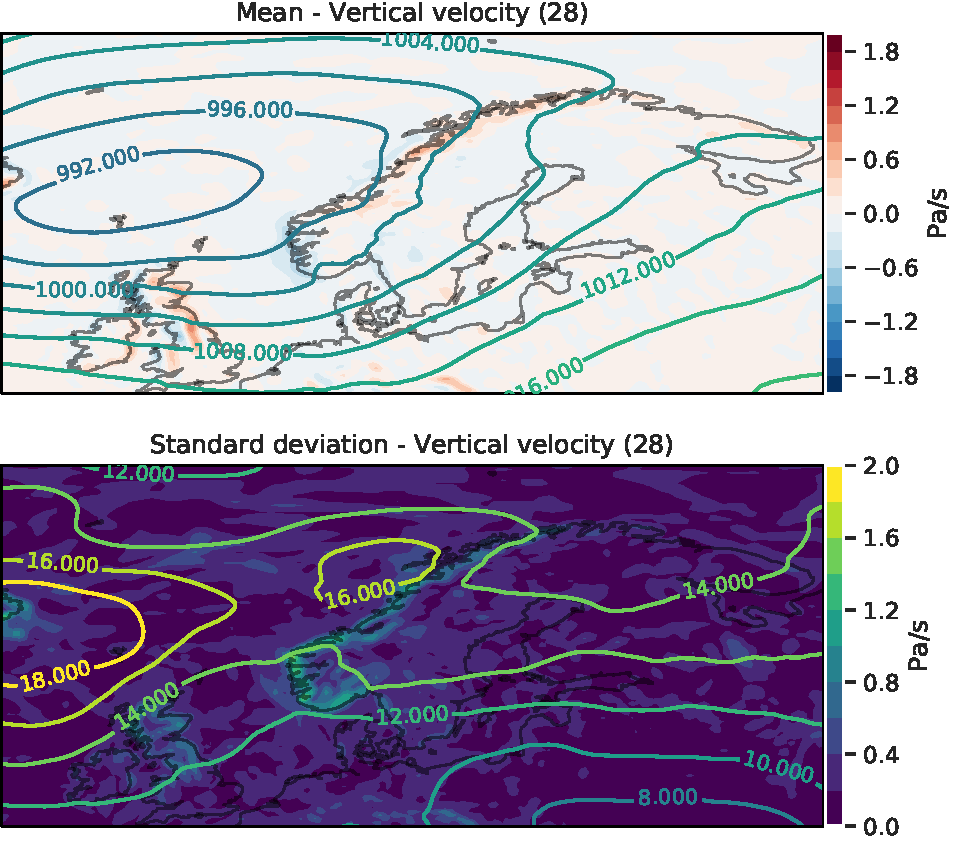
\includegraphics[width=\textwidth]{Figures/WENZV.pdf}
         \caption{Vertical velocity for cases at Sola}
         \label{fig:ENZVW}
     \end{subfigure}
    \begin{subfigure}[b]{0.5\textwidth}
    \centering
    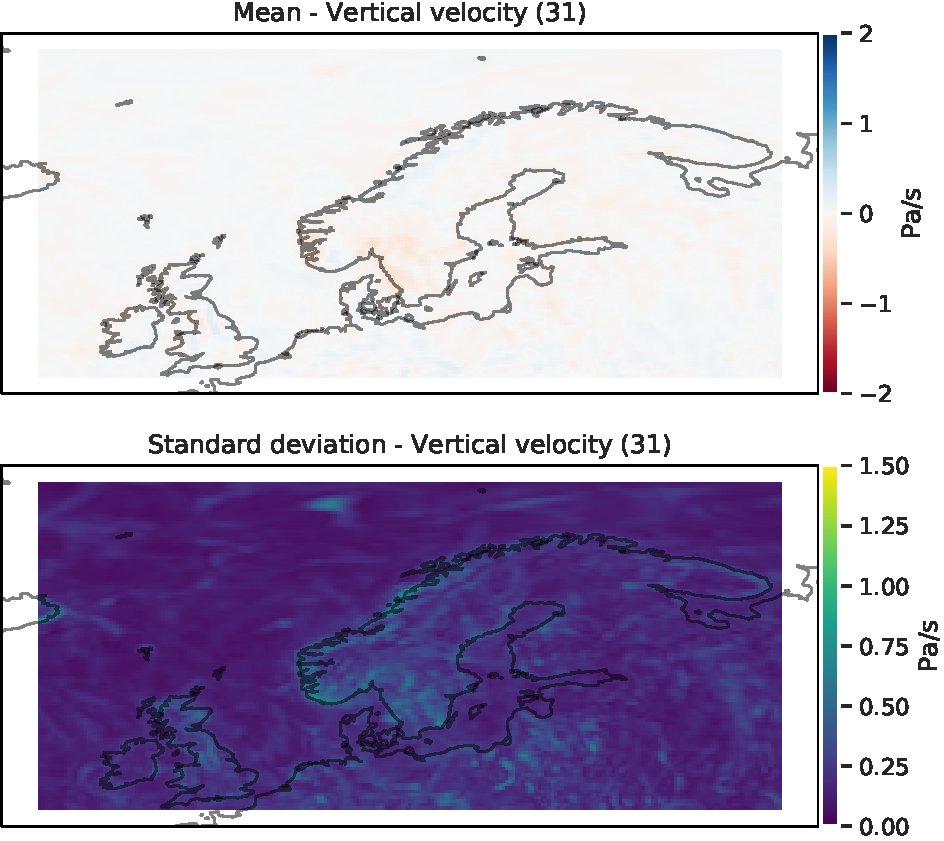
\includegraphics[width=\textwidth]{Figures/WENGM.pdf}
    \caption{Vertical velocity for cases in Gardermoen zone.}
    \label{fig:ENGMW}
\end{subfigure}
\caption{Same as Figure \ref{fig:verticalzones}, but for only the biggest airports.}
\label{fig:verticalairports}
\end{figure}


\subsection{Different types of precipitation for triggered lightning events}
The ERA5 reanalysis model differentiates between convective precipitation arising from the convection scheme in the integrated forecasting system and large scale precipitation arising from the cloud scheme in the integrated forecasting system. To investigate the atmospheric conditions, this thesis divides into these two different categories of precipitation to distinguish between large scale and locally caused precipitation.

\subsubsection{Large scale precipitation}
Figure \ref{fig:largescalezones} shows no clear sign of large scale precipitation being present anywhere but the west coast of Norway. However, for \textit{all} the composites (all zones), only the west coast has substantial amounts of large scale precipitation. This is further reinforced when looking at the case for Flesland and Sola in Figure \ref{fig:largescaleairports}. Again, Gardermoen sticks out due to not having any clear sign of large scale precipitation neither at the west coast nor around Gardermoen. This can again be explained by Gardermoen predominantly having triggered lightning events during summertime.

\begin{figure}
\begin{subfigure}[b]{0.49\textwidth}
    \centering
    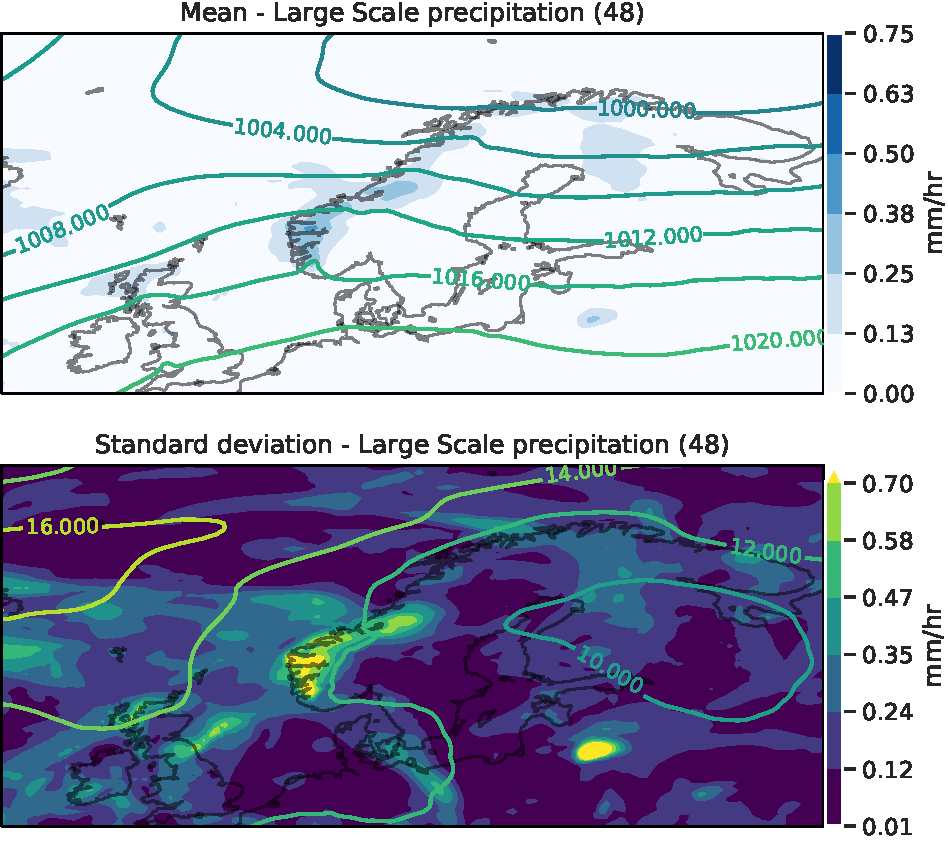
\includegraphics[width=\textwidth]{Figures/lsPNord.pdf}
    \caption{Large scale for cases in North zone.}
    \label{fig:NordlsP}
\end{subfigure}
\begin{subfigure}[b]{0.49\textwidth}
    \centering
    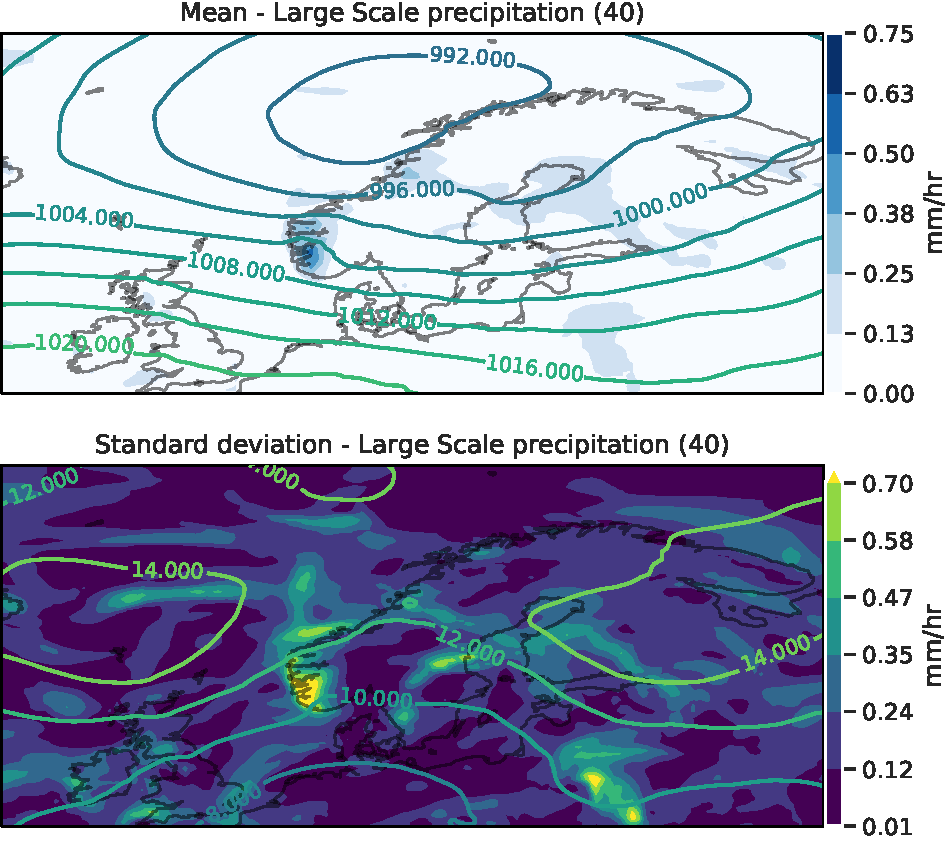
\includegraphics[width=\textwidth]{Figures/lsPNordvest.pdf}
    \caption{Large scale precipitation for cases in Northwest zone.}
    \label{fig:NordWestlsP}
\end{subfigure}
\begin{subfigure}[b]{0.49\textwidth}
    \centering
    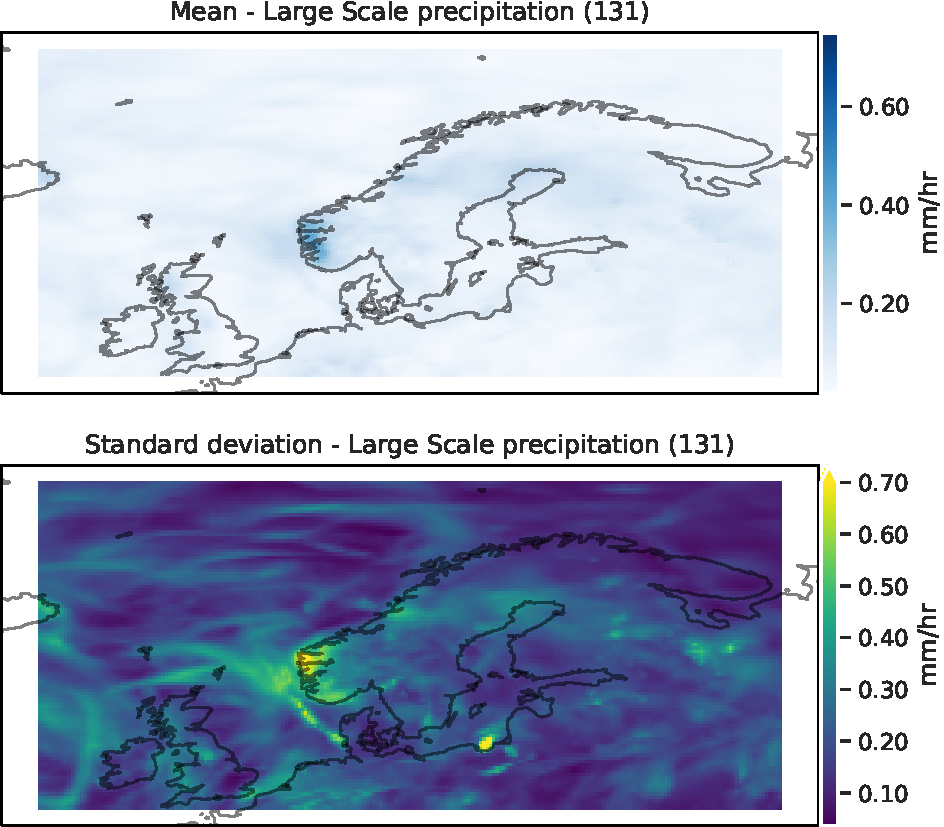
\includegraphics[width=\textwidth]{Figures/lsPVest.pdf}
    \caption{Large scale precipitation for cases in West zone.}
    \label{fig:WestlsP}
\end{subfigure}
\begin{subfigure}[b]{0.49\textwidth}
    \centering
    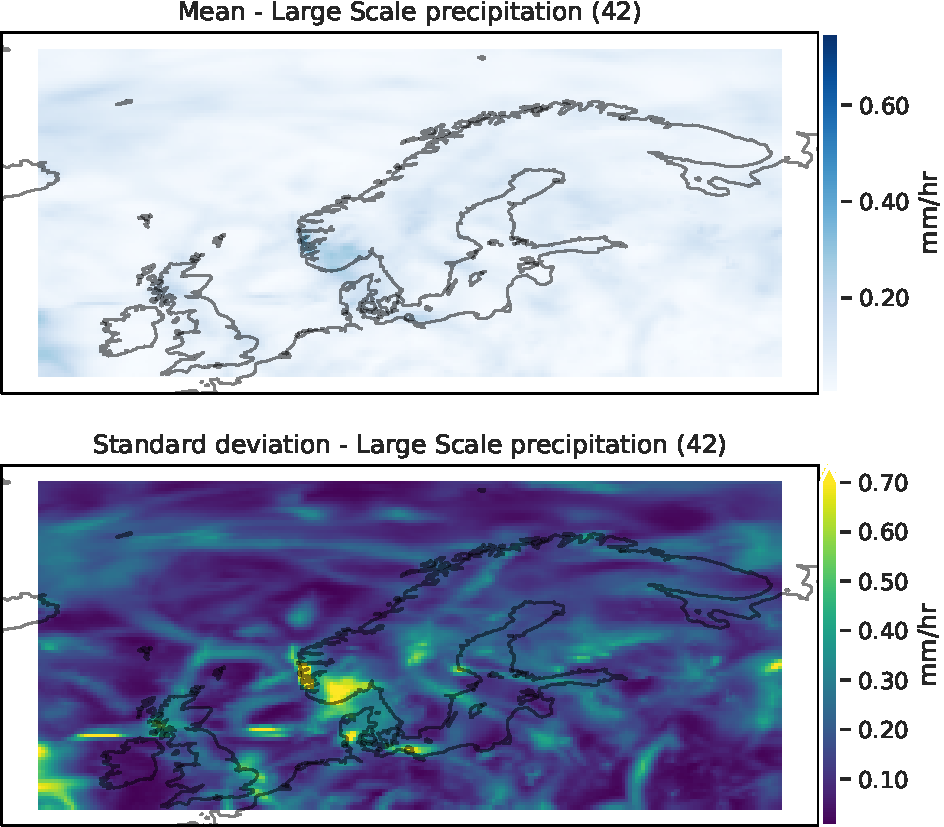
\includegraphics[width=\textwidth]{Figures/lsPSor.pdf}
    \caption{Large scale precipitation for cases in South zone.}
    \label{fig:SouthlsP}
\end{subfigure}
\caption{Large scale precipitation composites for both \acrshort{htl} and \acrshort{fwtl} cases in different geographical zones. Included are cases where height information was \textit{not} provided in the Avinor data set.}
\label{fig:largescalezones}
\end{figure}

\begin{figure}
     \centering
     \begin{subfigure}[b]{0.49\textwidth}
         \centering
         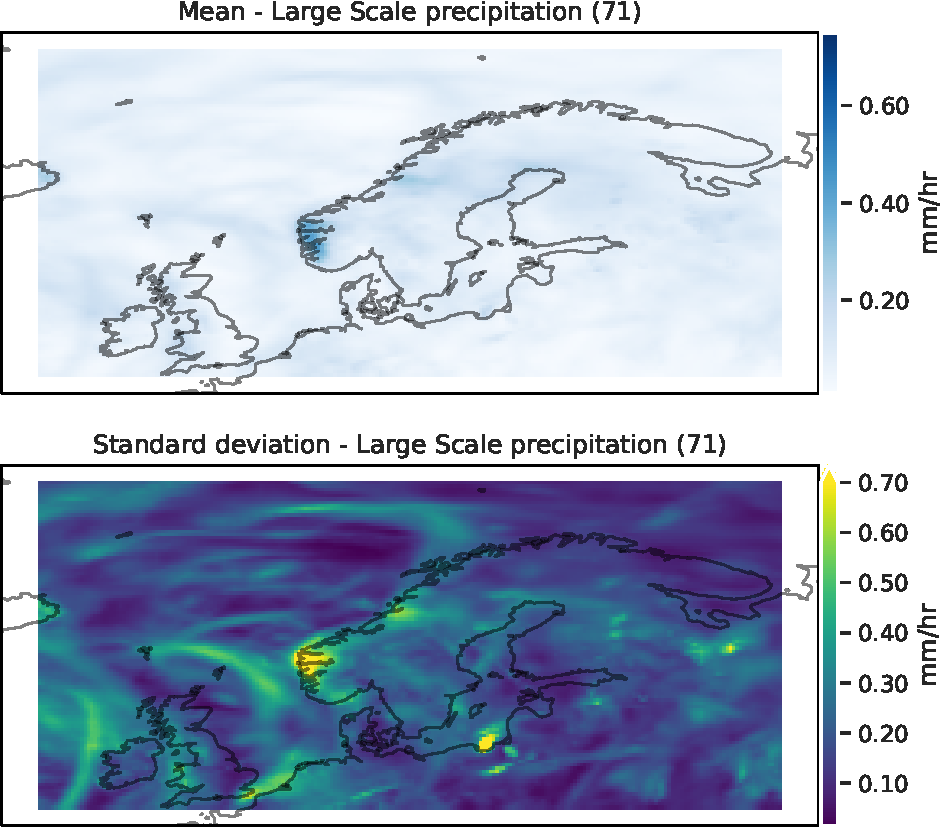
\includegraphics[width=\textwidth]{Figures/lsPENBR.pdf}
         \caption{Large scale precipitation for cases at  Flesland.}
         \label{fig:ENBRlsP}
     \end{subfigure}
     \hfill
     \begin{subfigure}[b]{0.49\textwidth}
         \centering
         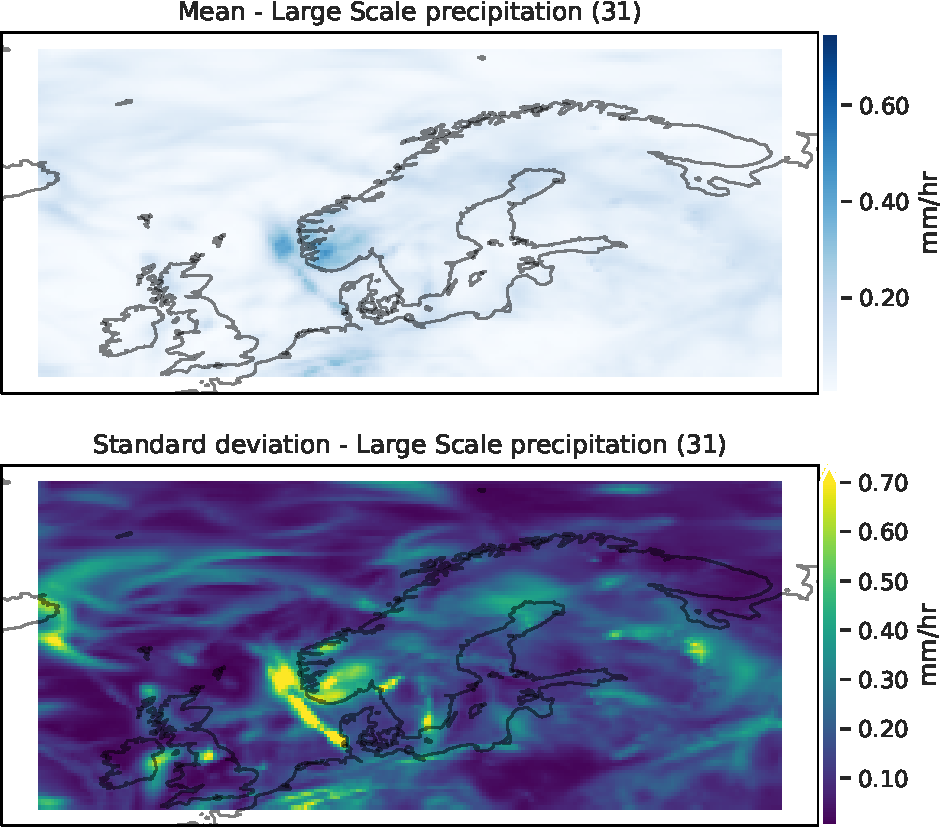
\includegraphics[width=\textwidth]{Figures/lsPENZV.pdf}
         \caption{Large scale precipitation for cases at Sola.}
         \label{fig:ENZVlsP}
     \end{subfigure}

    \begin{subfigure}[b]{0.5\textwidth}
    \centering
    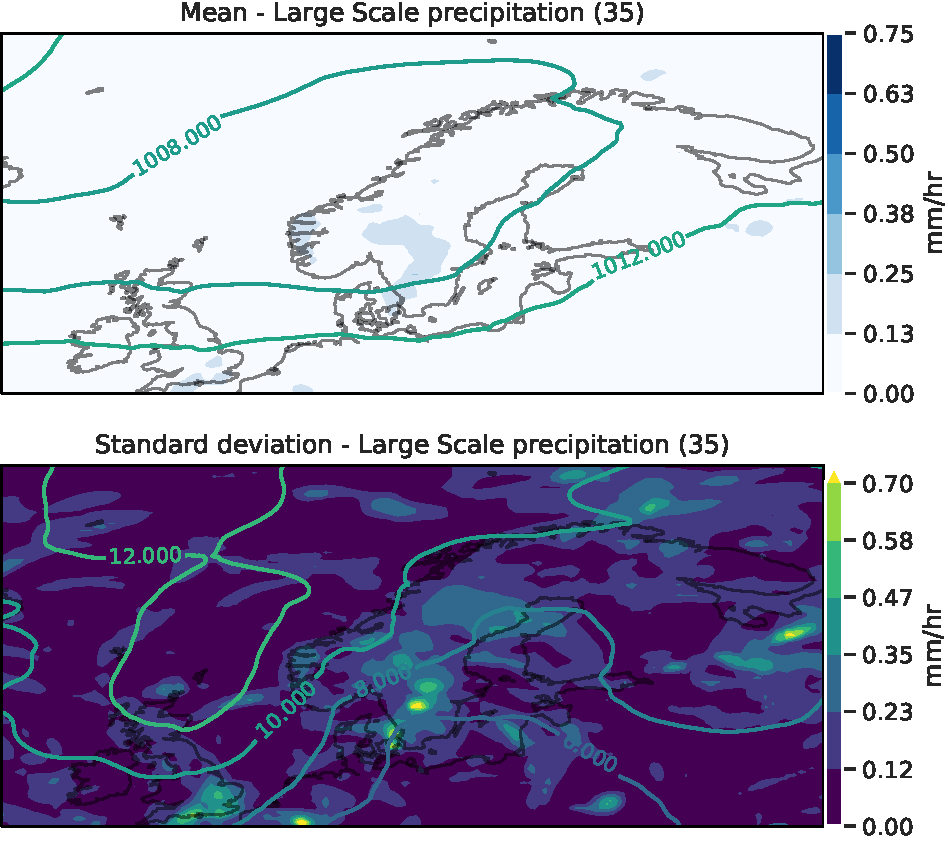
\includegraphics[width=\textwidth]{Figures/lsPENGM.pdf}
    \caption{Large scale precipitation for cases at Gardermoen.}
    \label{fig:ENGMlsP}
\end{subfigure}
\caption{Same as for Figure \ref{fig:largescalezones}, but for only the biggest airports}
\label{fig:largescaleairports}
\end{figure}

\subsubsection{Convective precipitation}
Now, considering the convective precipitation as shown in Figure \ref{fig:convectivezones}, there are clear convective systems precipitating in all zones, even in the South zone. The standard deviation is also somewhat high, but this is to be expected when considering the chaotic nature of convective precipitation. This standard deviation is also higher than the mean value in some cases, which also hints to a problem of placing convective scale systems, as was the case for the coastal zones discussed in Section \ref{sec:verticalvelocity}. The cases near the airports are shown in Figure \ref{fig:convectiveairports}. Flesland and Sola show the same picture as the previous figure in that there is a large precipitation intensity along the west coast, but high standard deviation, especially around Sola in the Sola case and around Flesland in the Flesland case. Here, Gardermoen also has very clearly convective precipitation related to the triggered lightning events. 

\begin{figure}
\begin{subfigure}[b]{0.49\textwidth}
    \centering
    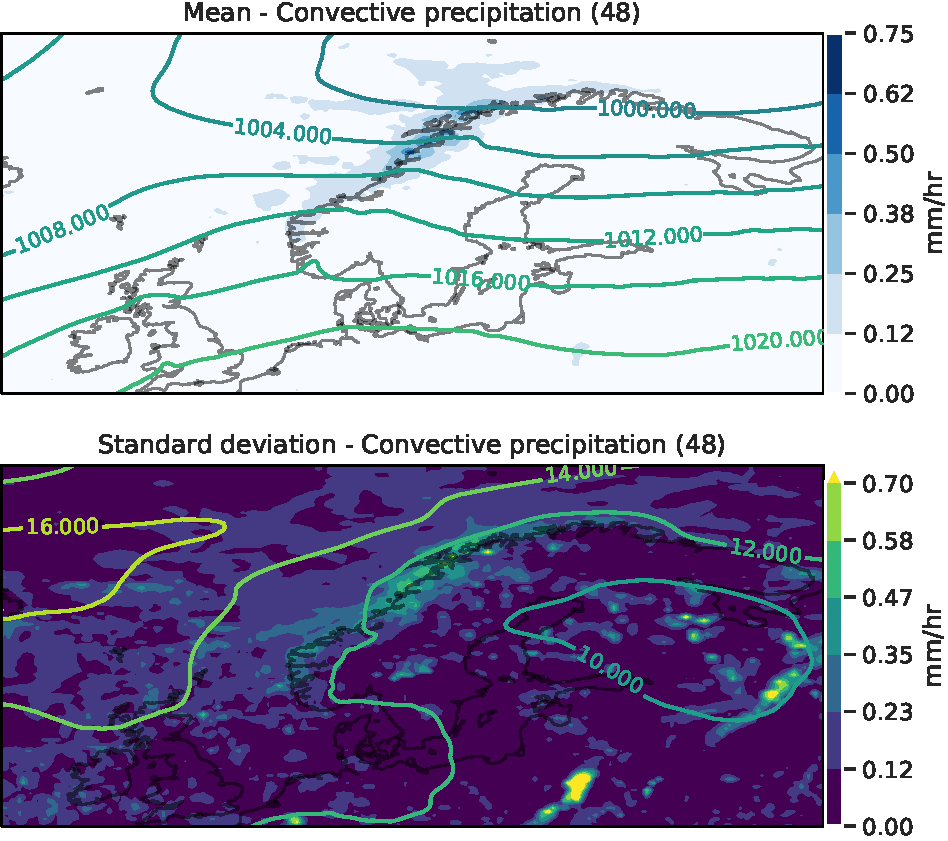
\includegraphics[width=\textwidth]{Figures/cPNord.pdf}
    \caption{Convective precipitation for cases in North zone.}
    \label{fig:NordcP}
\end{subfigure}
\begin{subfigure}[b]{0.49\textwidth}
    \centering
    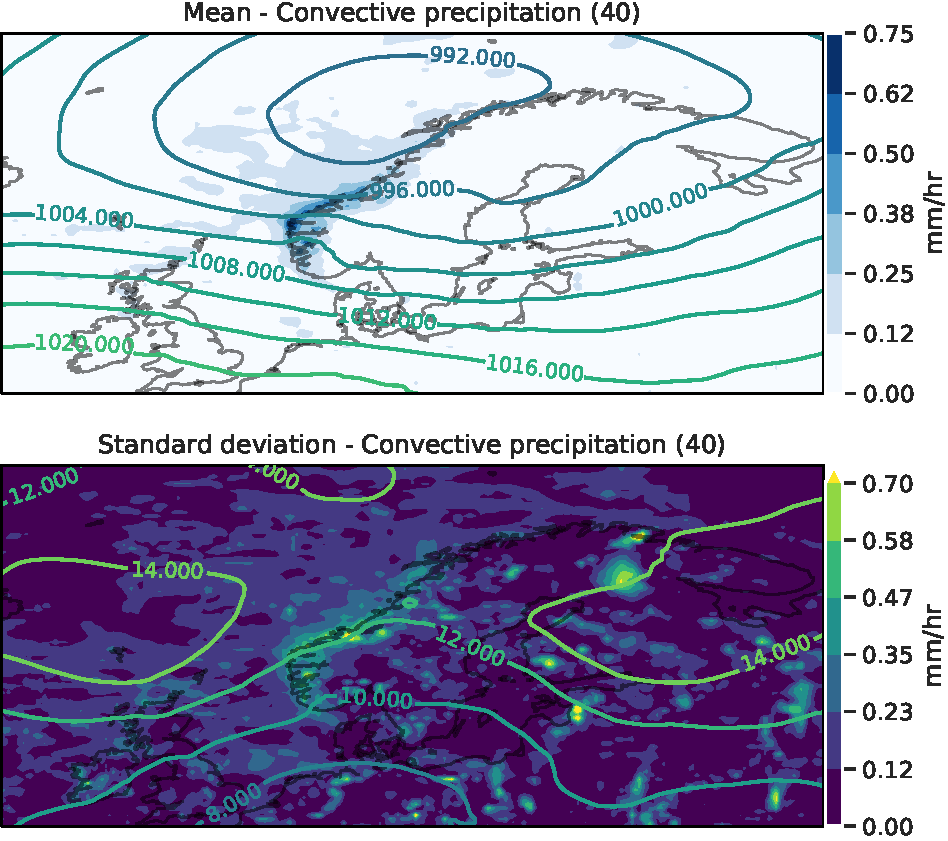
\includegraphics[width=\textwidth]{Figures/cPNordvest.pdf}
    \caption{Convective precipitation for cases in Northwest zone.}
    \label{fig:NordWestcP}
\end{subfigure}
\begin{subfigure}[b]{0.49\textwidth}
    \centering
    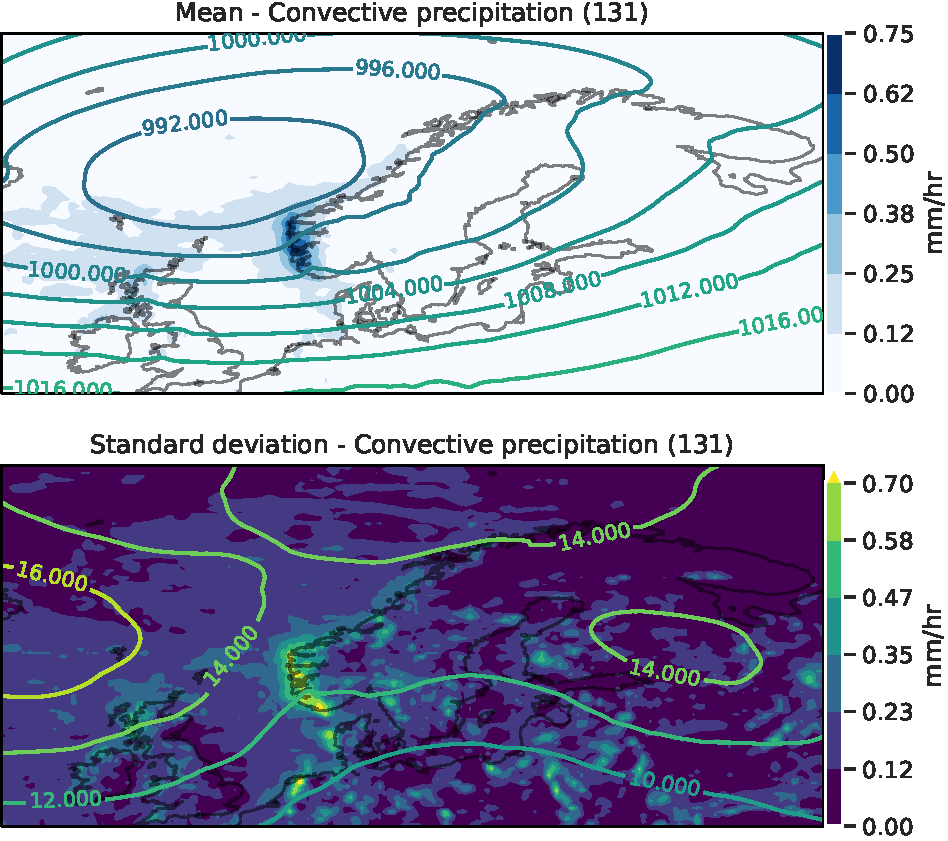
\includegraphics[width=\textwidth]{Figures/cPVest.pdf}
    \caption{Convective precipitation for cases in West zone.}
    \label{fig:WestcP}
\end{subfigure}
\begin{subfigure}[b]{0.49\textwidth}
    \centering
    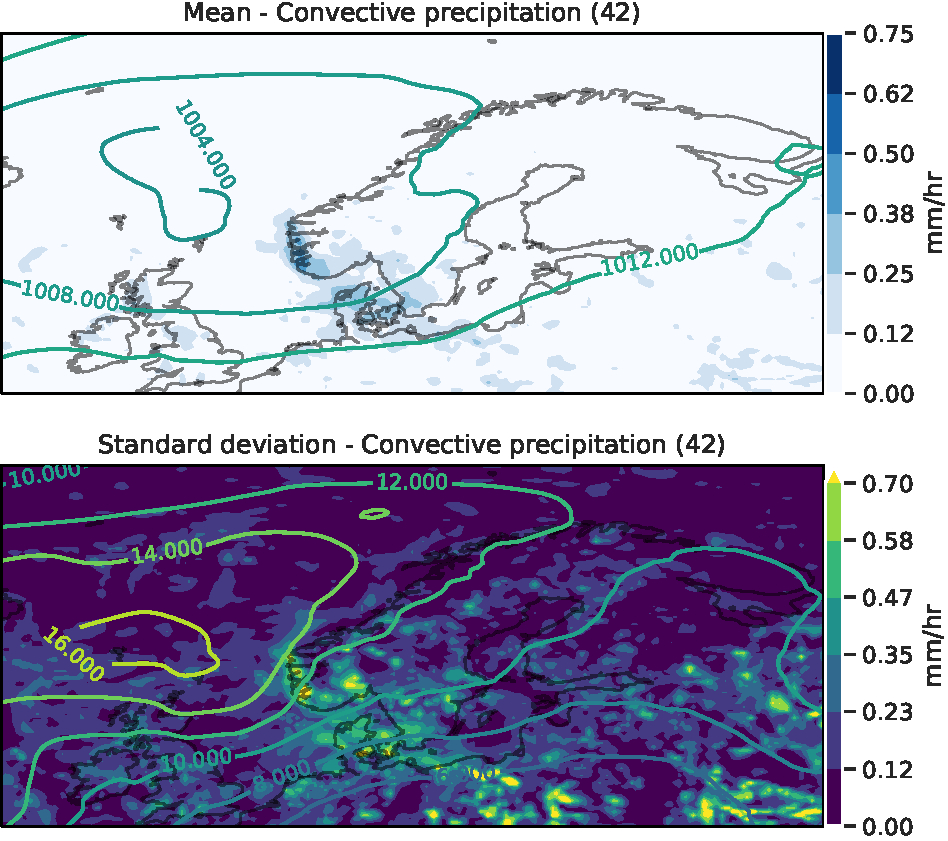
\includegraphics[width=\textwidth]{Figures/cPSor.pdf}
    \caption{Convective precipitation for cases in South zone.}
    \label{fig:SouthcP}
\end{subfigure}
\caption{Convective precipitation composites for the different zones}
\label{fig:convectivezones}
\end{figure}

\begin{figure}
     \centering
     \begin{subfigure}[b]{0.49\textwidth}
         \centering
         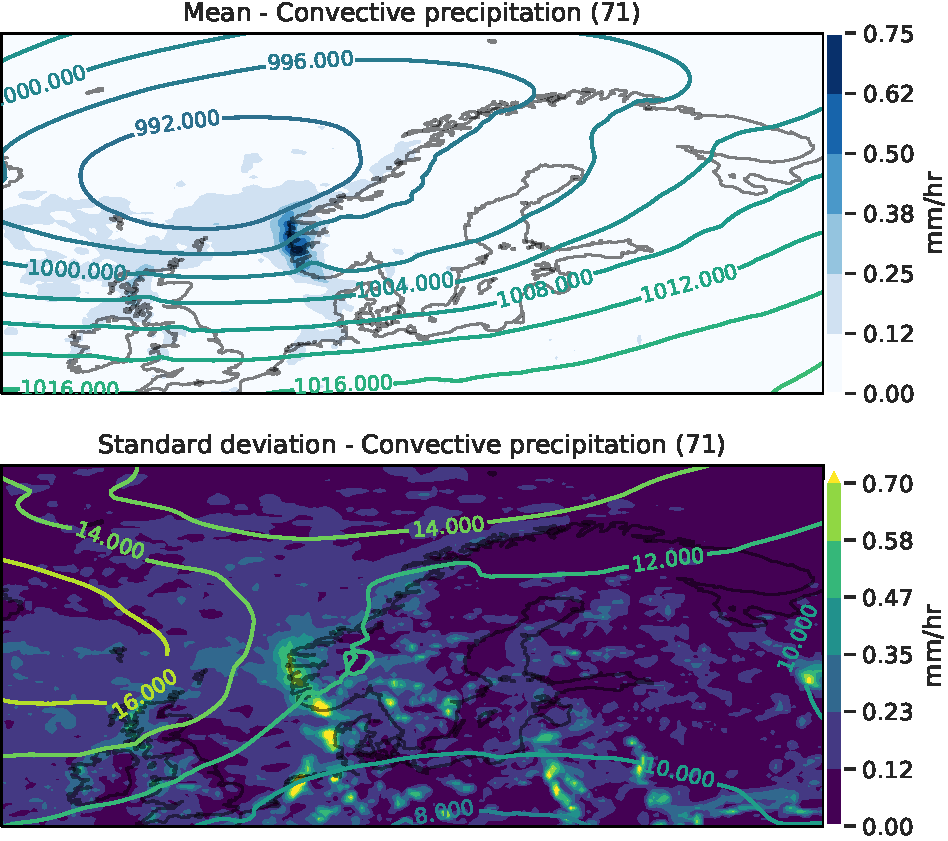
\includegraphics[width=\textwidth]{Figures/cPENBR.pdf}
         \caption{Convective precipitation for cases at Flesland}
         \label{fig:ENBRcP}
     \end{subfigure}
     \hfill
     \begin{subfigure}[b]{0.49\textwidth}
         \centering
         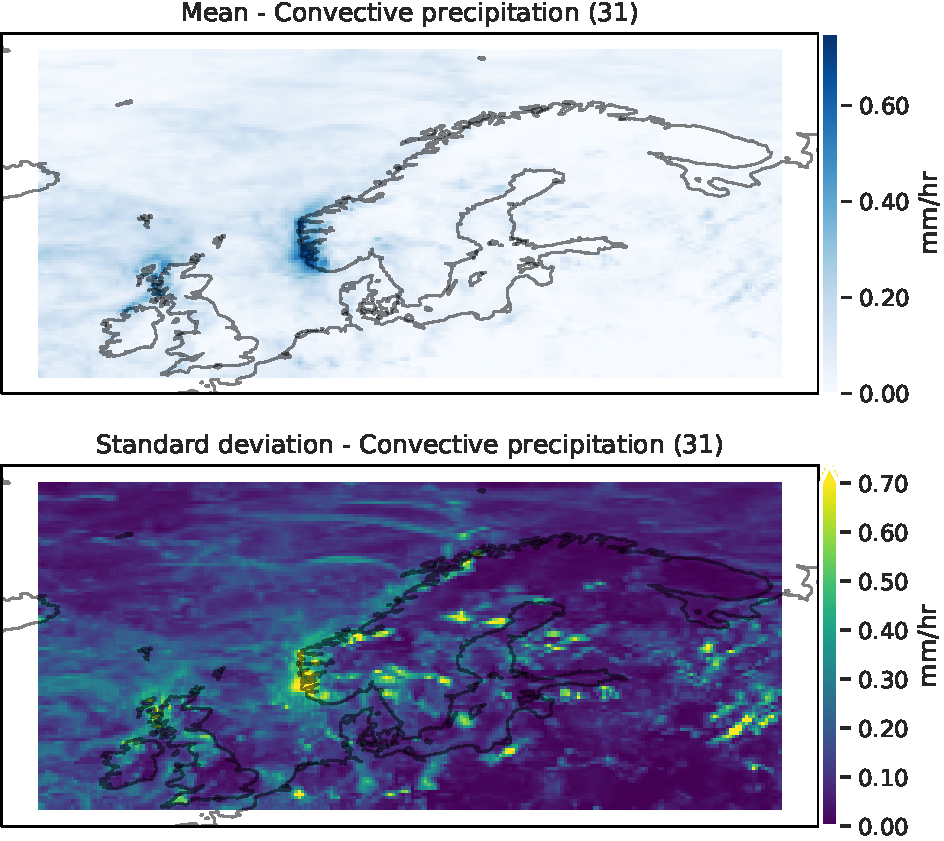
\includegraphics[width=\textwidth]{Figures/cPENZV.pdf}
         \caption{Convective precipitation for cases at Sola}
         \label{fig:ENZVcP}
     \end{subfigure}

    \begin{subfigure}[b]{0.5\textwidth}
    \centering
    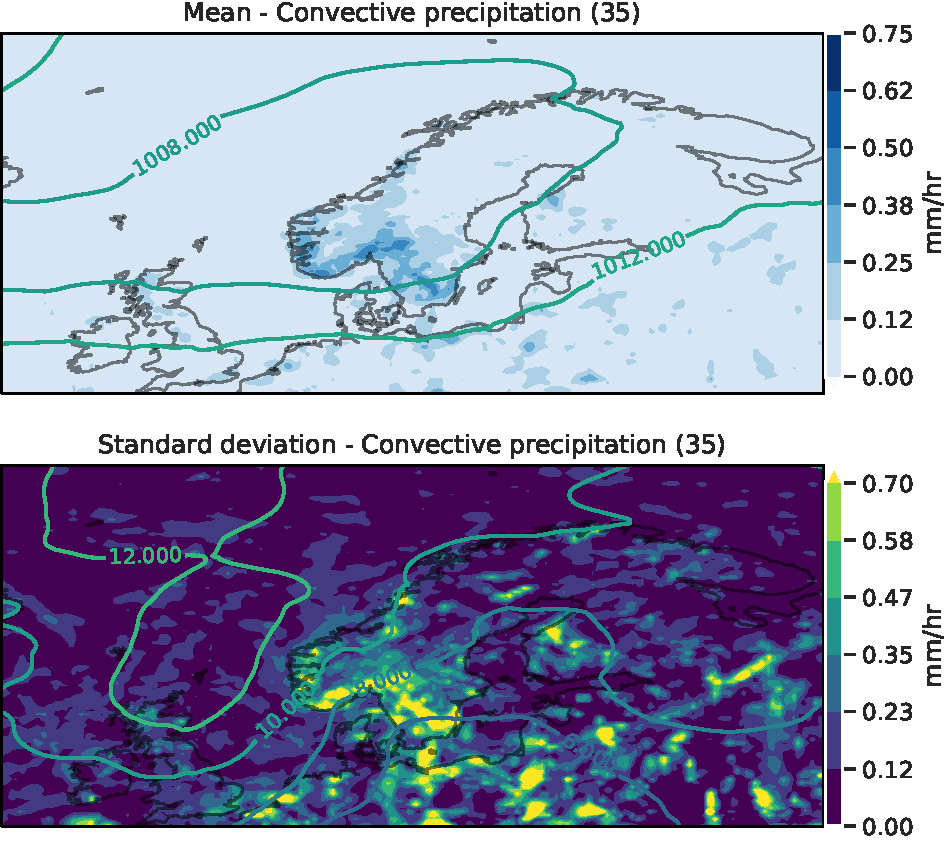
\includegraphics[width=\textwidth]{Figures/cPENGM.pdf}
    \caption{Convective precipitation for cases in Gardermoen zone.}
    \label{fig:ENGMcP}
\end{subfigure}
\caption{Convective precipitation composites for the biggest airports. }
\label{fig:convectiveairports}
\end{figure}

\section{What are the implications of the precipitation bug fix?}

To investigate this, Figure \ref{fig:fixeffect} shows the effect of considering hourly instead of accumulated precipitation\footnote{A map showing the }. Shown is an approximate halving of the frequency of Yellow risk for all airports. The higher risk categories (Orange and Red) are only substantially reduced at northfacing airports, i.e. airports in the northwest and North zone. Sola and Flesland see a halving in the Orange category, but not a substantial reduction in the Red. Flesland and Sola have approximately the same frequency of Red and Orange forecasts, but as shown in \ref{tab:traffic}, Flesland has double the amount of \acrshort{htl} and \acrshort{fwtl} cases.

To further investigate whether this leads to any reduction in \acrshort{hti} forecast skill, METAR data was considered to verify that \acrshort{hti} correctly identifies coastal and off-shore convective activity. Thus, the effect for the three airports from the North zone are shown in Figure \ref{fig:HTIMETAR1}. The figure shows a clear increase in frequency of non-White risk categories for all three airports. Hammerfest and Bodø have a slight increase in \acrshort{htl}-related phenomena forecasted as White (Here, snow and showers.) However, there is also some reduction in other phenomena such that this seems to be a non-substantial increase. The same is observed for Figure \ref{fig:HTIMETAR2}, which shows the risk categories for the three northwestern coastal airports: a clear increase in frequency of non-White risk categories when convective activity is observed. It should be noted that there seems to be no clear total increase or decrease in the White category for all three airports. In all, the skill of the \acrshort{hti} does not seem to be reduced, but rather increased by taking into account the hourly precipitation. %The argument for a reduction can be made, due to a known bug in the HARMONIE-configuration used at MEPS, leading to an underrepresentation of precipitation along the coast of Norway. \cite{Morten_private}

\begin{figure}
    \centering
     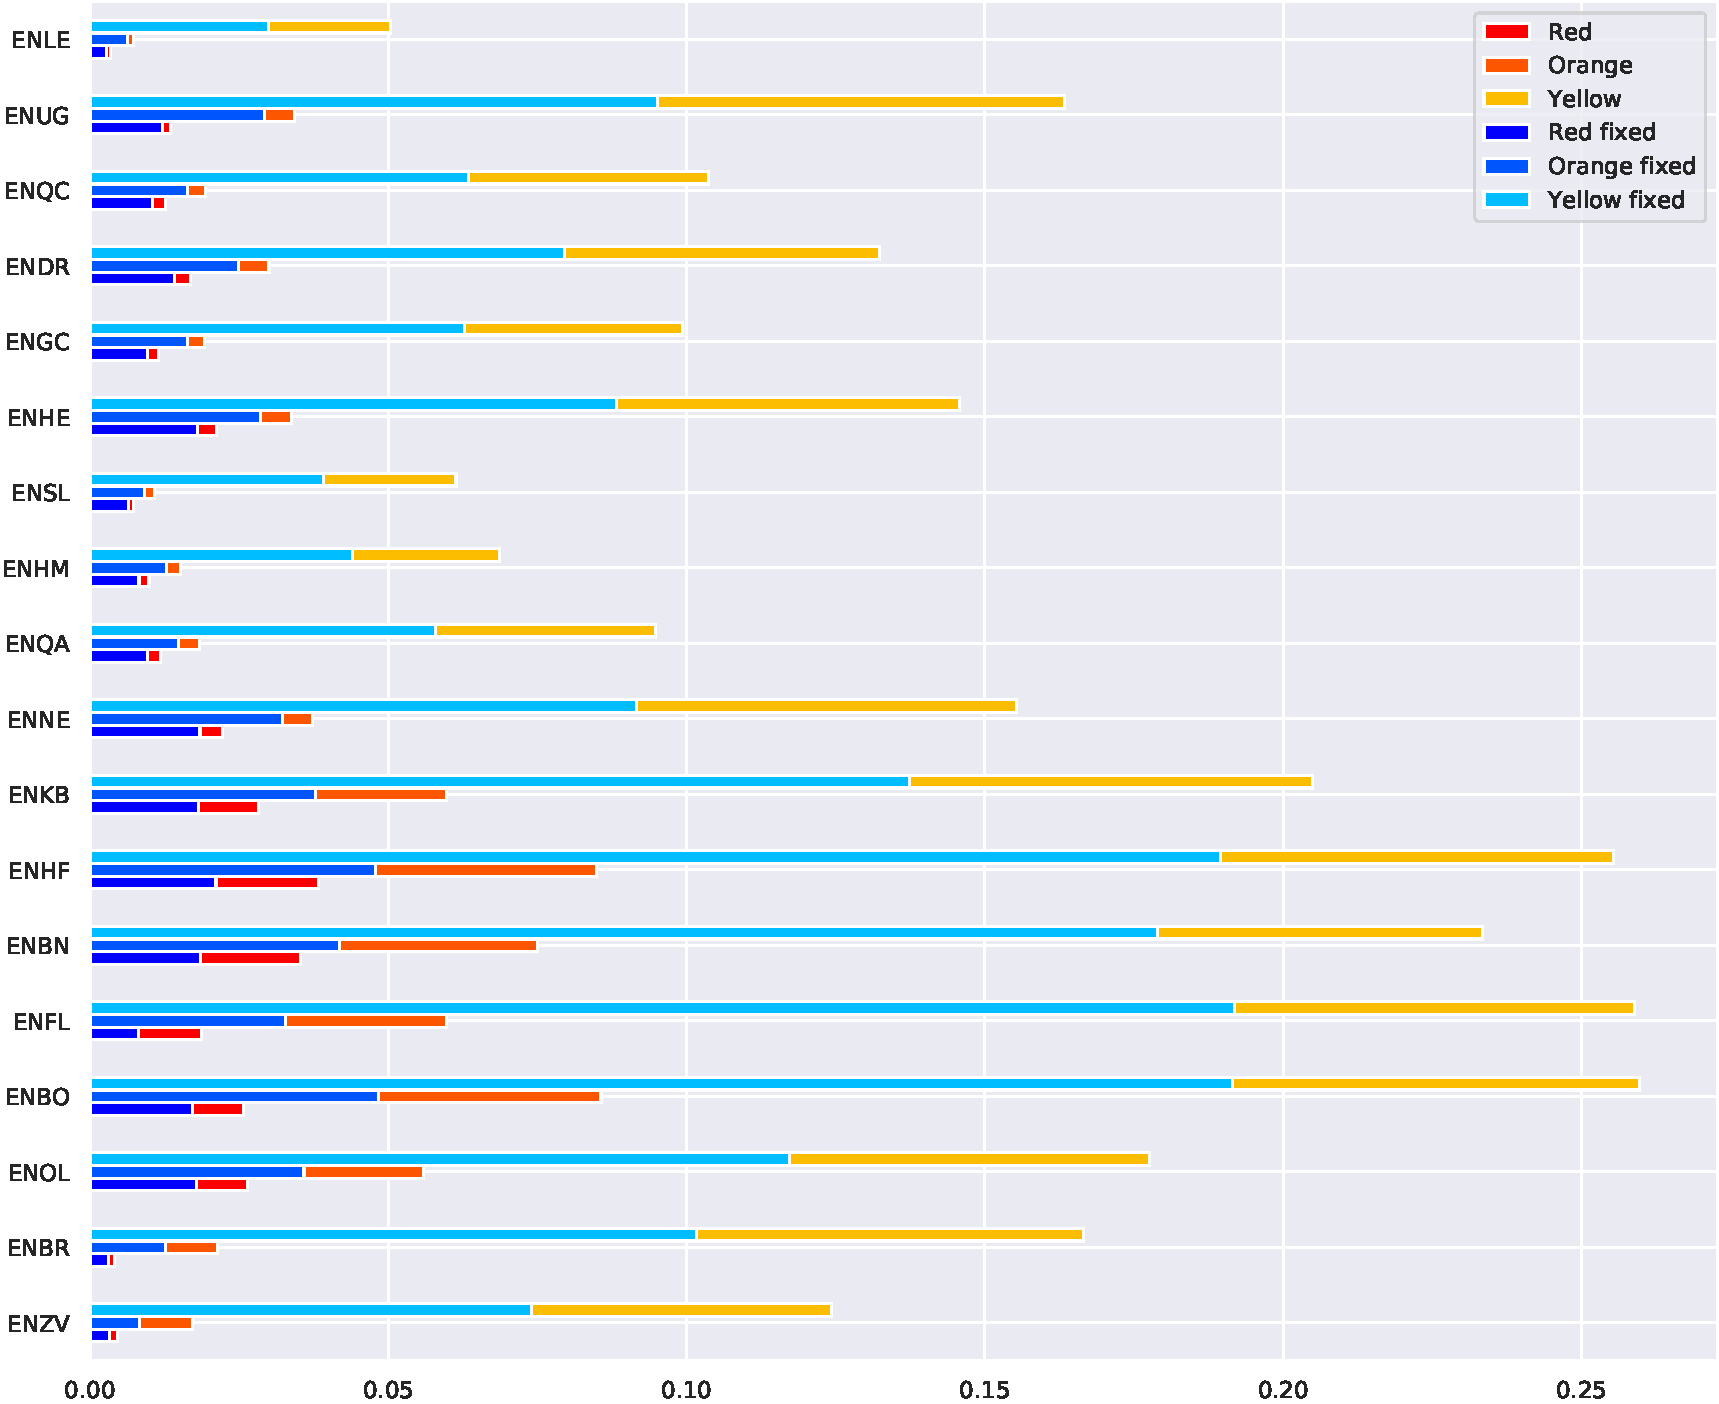
\includegraphics[width=\textwidth]{Figures/fixeffect.pdf}
    \caption{Frequency of \acrshort{hti}-risk levels during \acrshort{htl}-season (October-April), before and after fixing the erroneous forecast, for selected airports.}
    \label{fig:fixeffect}
\end{figure}

\begin{figure}
    \centering
    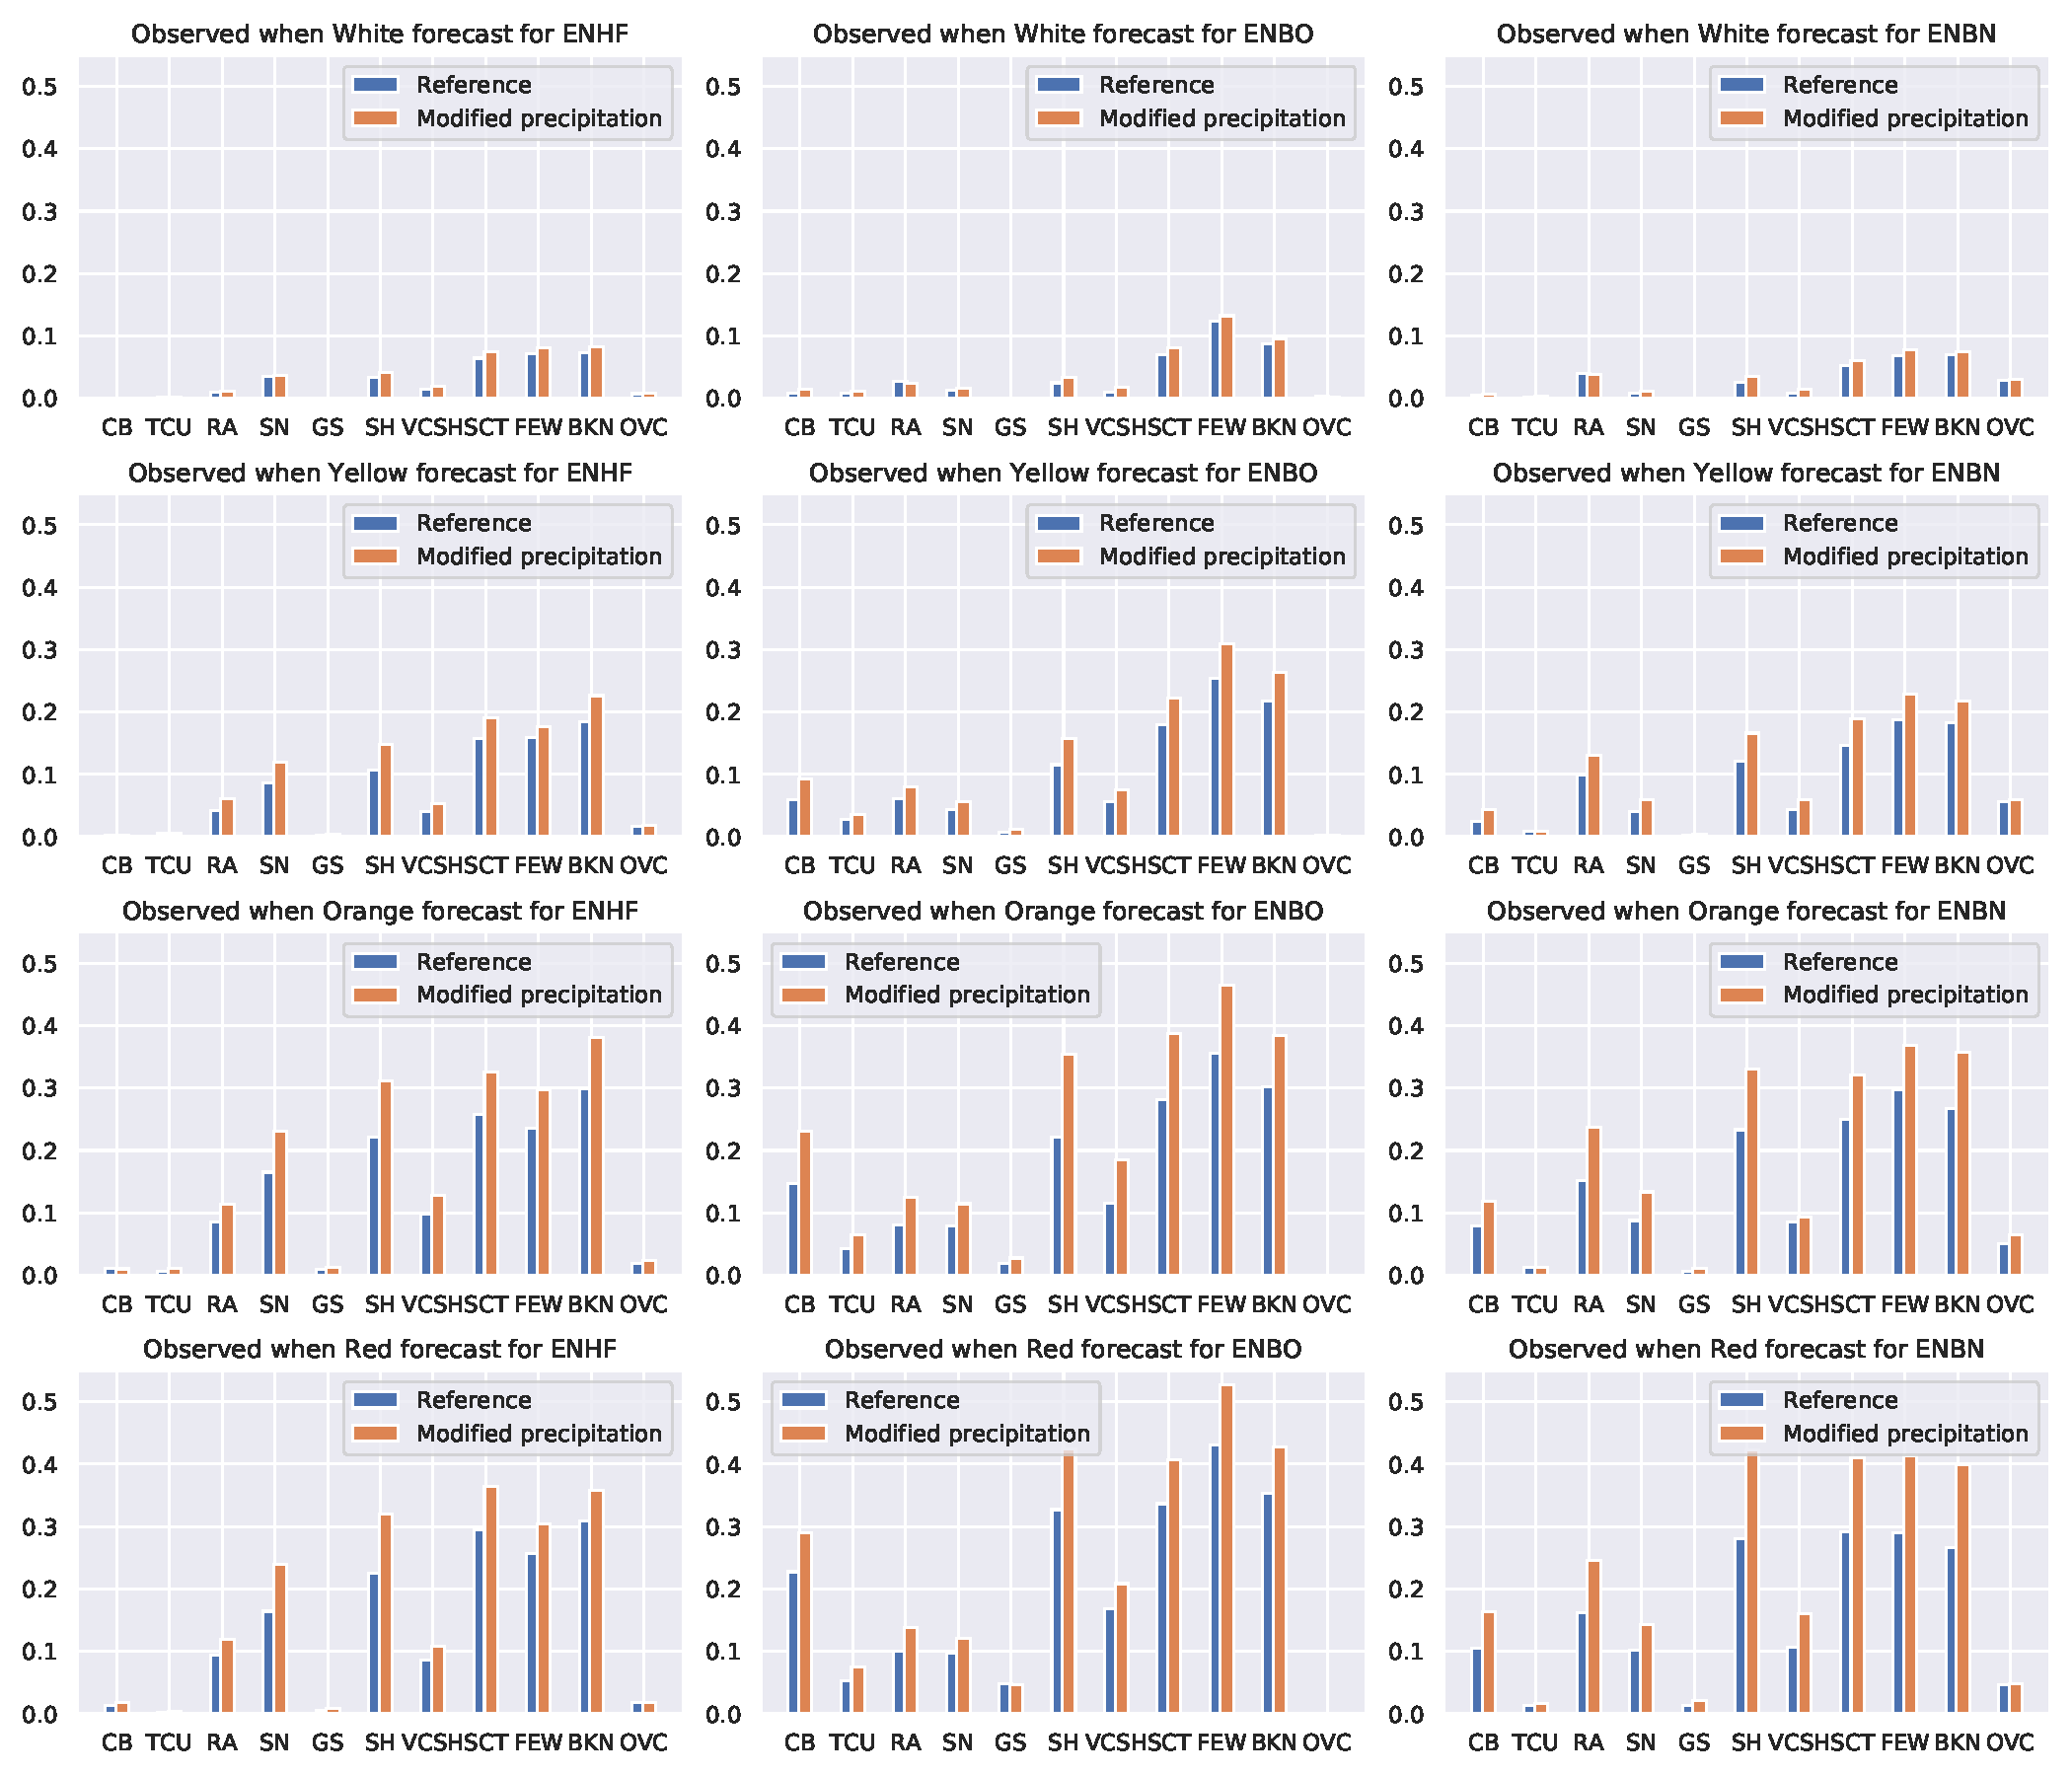
\includegraphics[width=\textwidth]{Figures/HTIMetar1.pdf}
    \caption{Frequency of \acrshort{hti}-risk given observed meteorological-phenomenon during \acrshort{htl}-season (October-April), for the three northernmost coastal airports: Hammerfest (ENHF), Bodø (ENBO), and Brønnøysund (ENBN)}
    \label{fig:HTIMETAR1}
\end{figure}

\begin{figure}
    \centering
    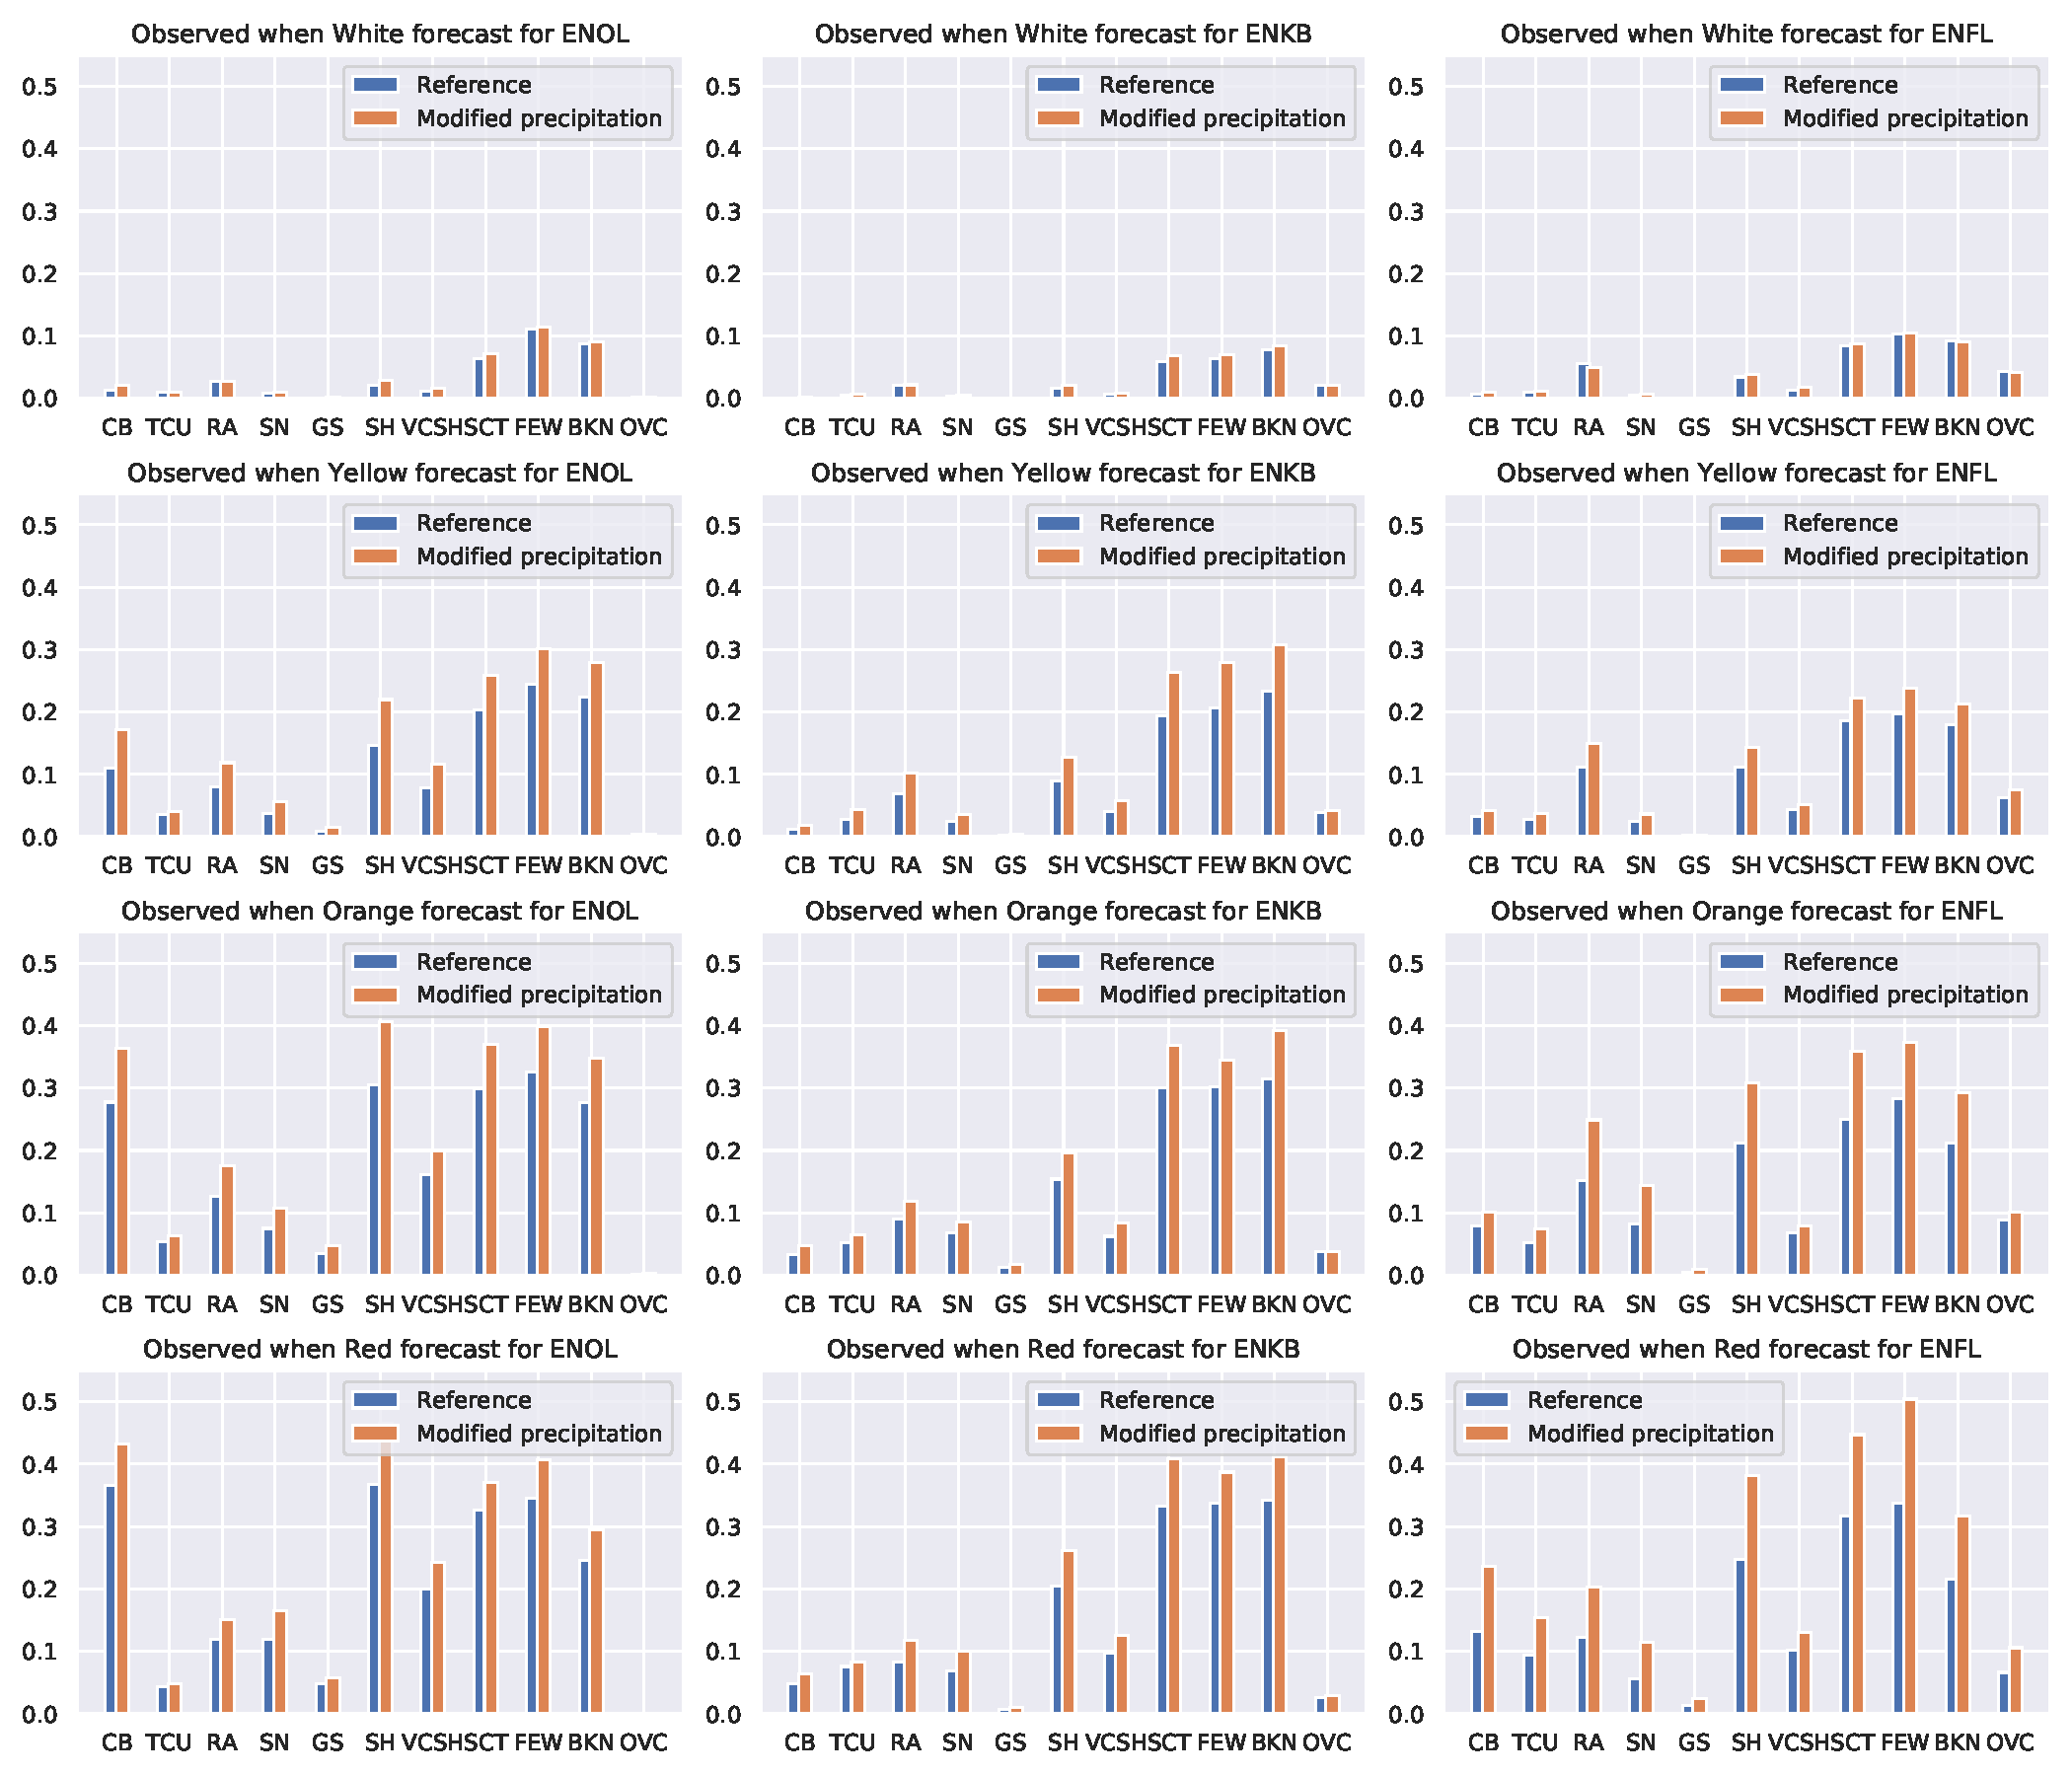
\includegraphics[width=\textwidth]{Figures/HTIMetar2.pdf}
    \caption{Frequency of \acrshort{hti}-risk given observed meteorological-phenomenon during \acrshort{htl}-season (October-April), for the three northwestern coastal airports: Ørlandet (ENOL), Kristiansund (ENKB), and Florø (ENFL)}
    \label{fig:HTIMETAR2}
\end{figure}


\section{How do the sub-indices perform during triggered lightning incidents?}
As discussed in Section \ref{sec:decomposition}, calculating sub-indices of forecasted \acrshort{hti} during recorded incidents allows for investigation into which, if any, of the sub-indices was under-evaluating the \acrshort{hti} risk. As stated in Section \ref{sec:hti}, \acrshort{hti} is calculated to be representative for the $750m$ ($\approx 2500$ feet) altitude. Thus, the following discussion only pertains to what is forecast at this altitude, and not (necessarily) at the height of the incident, as was done in Section \ref{sec:compositesera5}.

Figure \ref{fig:HeliAccum} shows 11 \acrshort{htl} cases from the Avinor data set with the sub-indices stacked on top of each other. On the x-axis is the altitude (in feet) at which the helicopter was flying. The figure shows the \acrshort{hti} to be at least $0.5$ for all 11 cases, but no cases were forecasted as Red and only two cases were forecasted as Orange. This is summarized in Table \ref{tab:HeliCont}. Figure \ref{fig:HeliDecomp} shows the sub-indices clearly delineated so that one can see which of the indices are lacking. The temperature sub-index is full for all but the third case, which, when calculated, had a temperature of -.67 $^{\circ}C$. Increasing the temperature to full would not increase the risk level in this case. Further, it can also be seen that in two of the 11 cases, precipitation would have been reduced to almost 0 if hourly instead of accumulated precipitation was considered, thus reducing the risk level to White. The third case where precipitation would be almost 0, was already White, so a reduction in risk level would not be seen. The most variability is found in the cloud and vertical velocity parameters. It should be noted that vertical velocity has had a positive value for all the cases, meaning that the upper threshold of the vertical velocity sub-index may be too strict. The cloud parameter reduces the risk level substantially (from Red to Yellow) for four of the cases. 

Looking now at the Fixed wing cases in \ref{fig:FWAccum}, which shows the total \acrshort{hti} decomposed to the sub-indices, with the altitude of the aircraft in feet on the x-axis. It can be seen that ten of the 34 cases would have a reduction in \acrshort{hti} due to consideration of the hourly (and not accumulated) precipitation. Only for three cases would this give a decrease in risk level. Even though some of these fixed wing incidents are happening at higher altitudes (e.g. 7000 feet), we see a relatively high sub-index for some of them, suggesting that there may be some convective activity in the whole column. This is also summarized in Table \ref{tab:FWCont}. Looking at Figure \ref{fig:FWDecomp}, one can see that vertical velocity is non-zero for \textit{all} cases, showing the vertical velocity to be positive in the case of triggered lightning events - even though many cases might be situated above or below the $750m$ altitude. The precipitation sub-index is generally not affected by differing heights, since it is a measure of how much precipitation would reach the ground - not precipitation in each level. The temperature sub-index shows a somewhat bad relation to the \acrshort{fwtl}. 19 of the cases had zero contribution from the temperature. This could be solely due to the aircraft being situated above or below the $750m$ altitude, but still close to the 0 $^{\circ}C$ isotherm.

It is to be noted from Tables \ref{tab:HeliCont} and \ref{tab:FWCont} that even though four fixed wing cases were correctly identified as Red, 41$\%$ were below the Yellow threshold. For the helicopter cases, zero were correctly identified as Red, but only two of the 11 (18.2$\%$) were below the Yellow threshold. Further, the helicopter data set is heavily influenced by the fact that they were recorded after the operational forecasting started: Any Red events were warned against and helicopter pilots have had an increased participation and reporting during this period. This may have lead to a skewing of the data set towards the tail of the majority of the cases, as seen in Figure \ref{fig:temperatureera5}, where the helicopter cases do not have a peak at the expected 0$^{\circ}C$ isotherm.

\begin{figure}
    \centering
    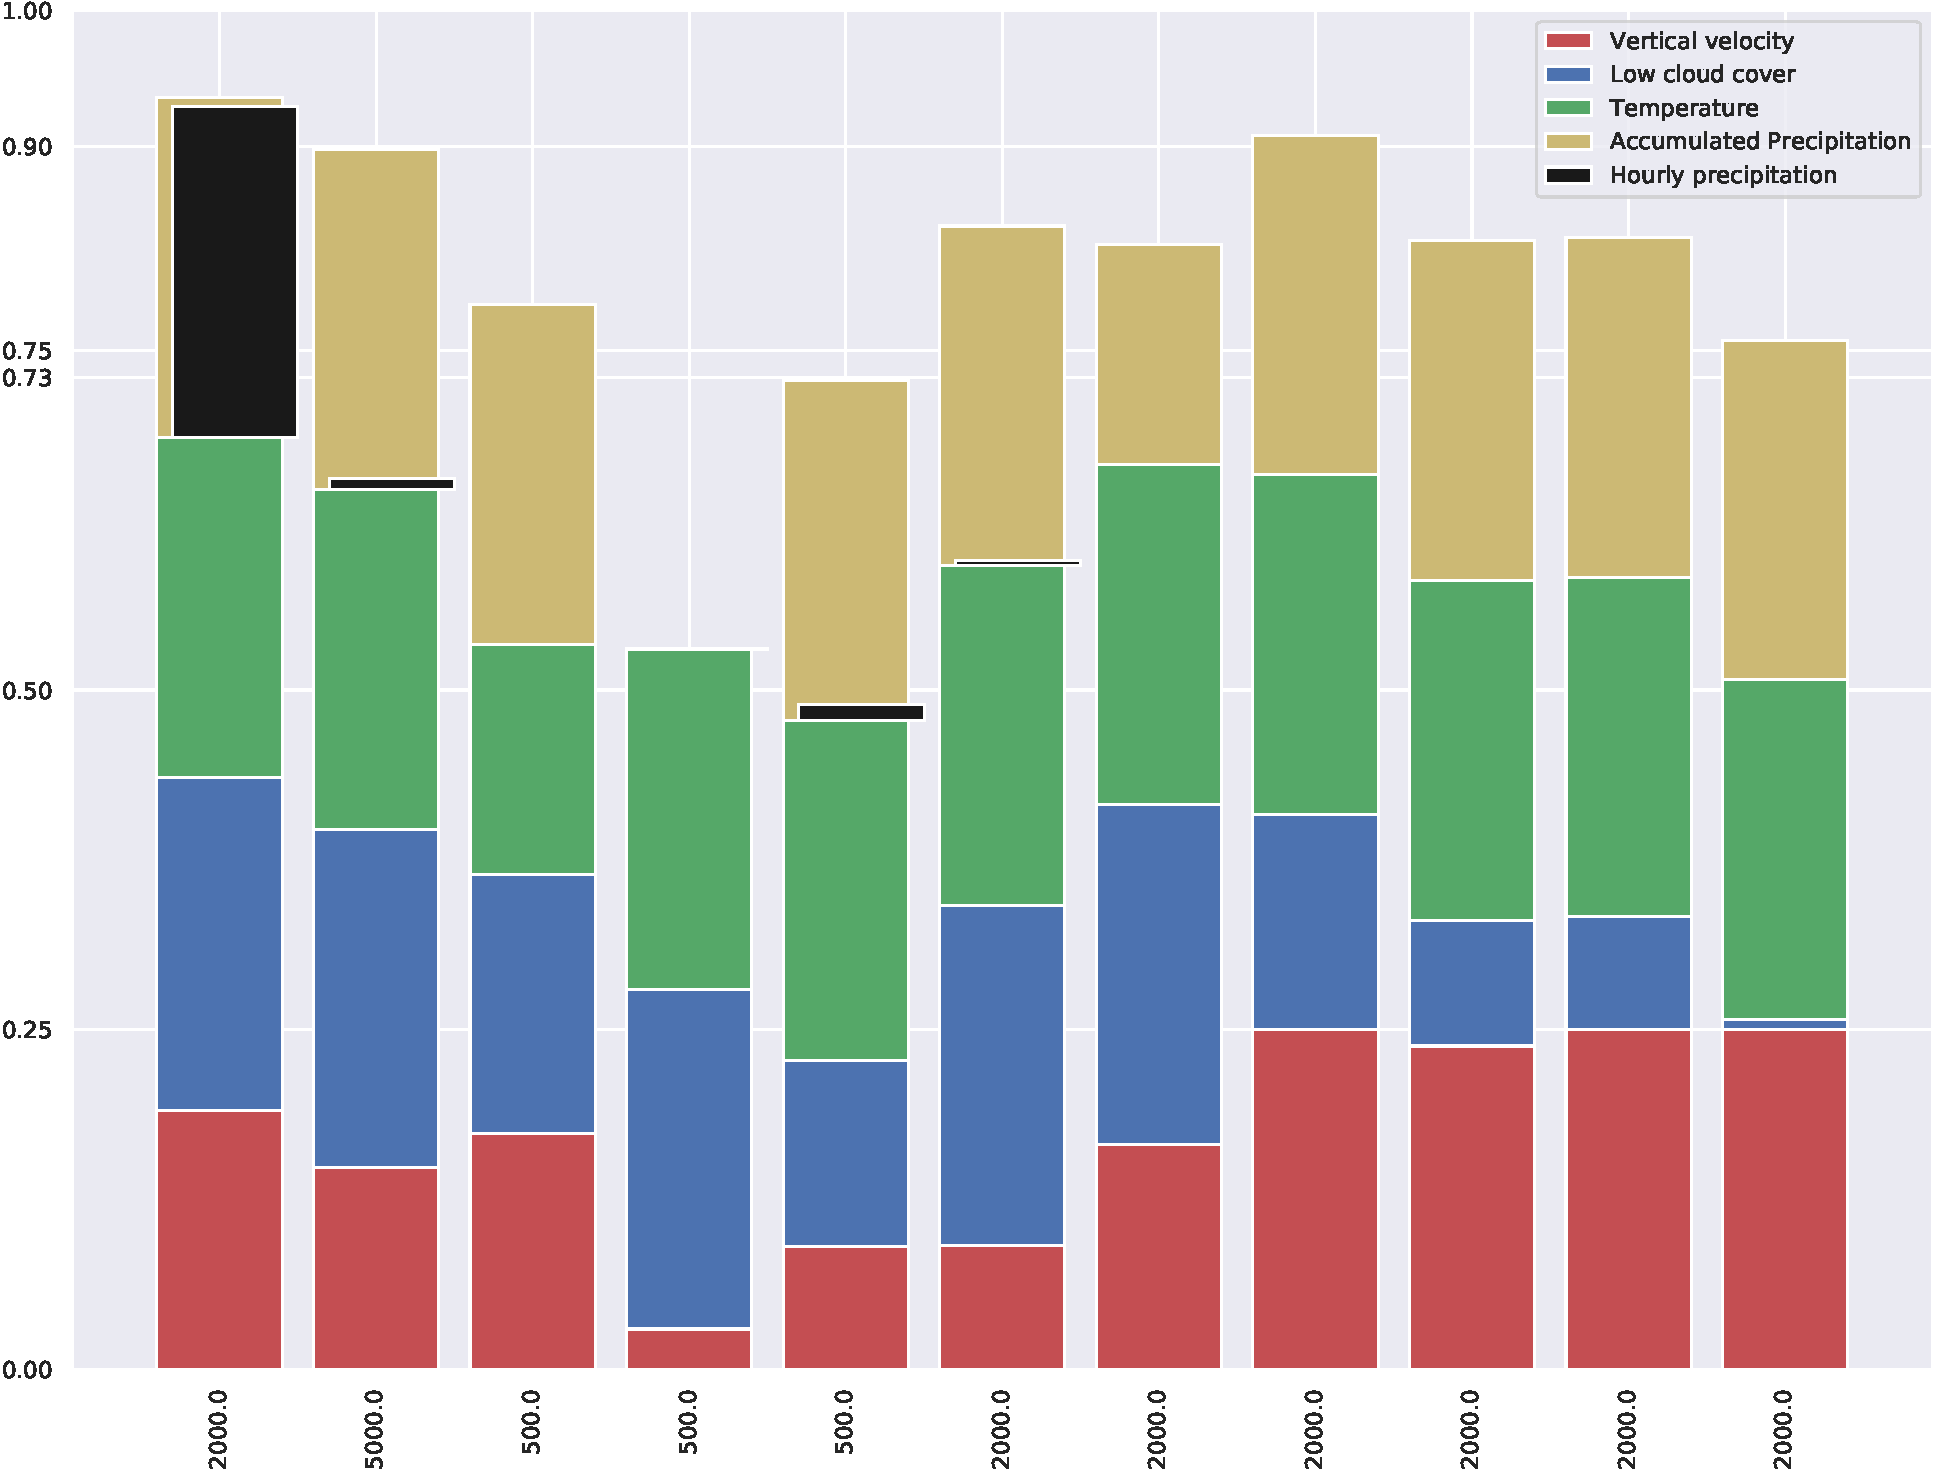
\includegraphics[width=\textwidth]{Figures/HeliAccum.pdf}
    \caption{Contributions from the different sub-indices, for Helicopter cases during the operational forecast. X-axis is height of incident in feet. Black on yellow is correction made by using the hourly precipitation instead of accumulated precipitation. Included are only cases from Avinor data set where position and height was available, for cases after November 2016.}
    \label{fig:HeliAccum}
\end{figure}

\begin{table}
    \centering
    \begin{tabular}{c|c|c|c}
        Forecast & With Accumulated & Without Accumulated & Missed (\%) \\ \hline
        >Yellow (0.73) & 9 & 7 & 2 (18.2\%)\\
        >Orange (0.90) & 2 & 2 & 7 (63.6\%)\\ 
        >Red (0.99) & 0 & 0 & 11 (100\%)\\
    \end{tabular}
    \caption{Amount of cases forecast in each risk category based on the $11$ Helicopter cases in Figure \ref{fig:HeliAccum}. A Red risk is counted in Orange, and Yellow.}
    \label{tab:HeliCont}
\end{table}

\begin{figure}
    \centering
    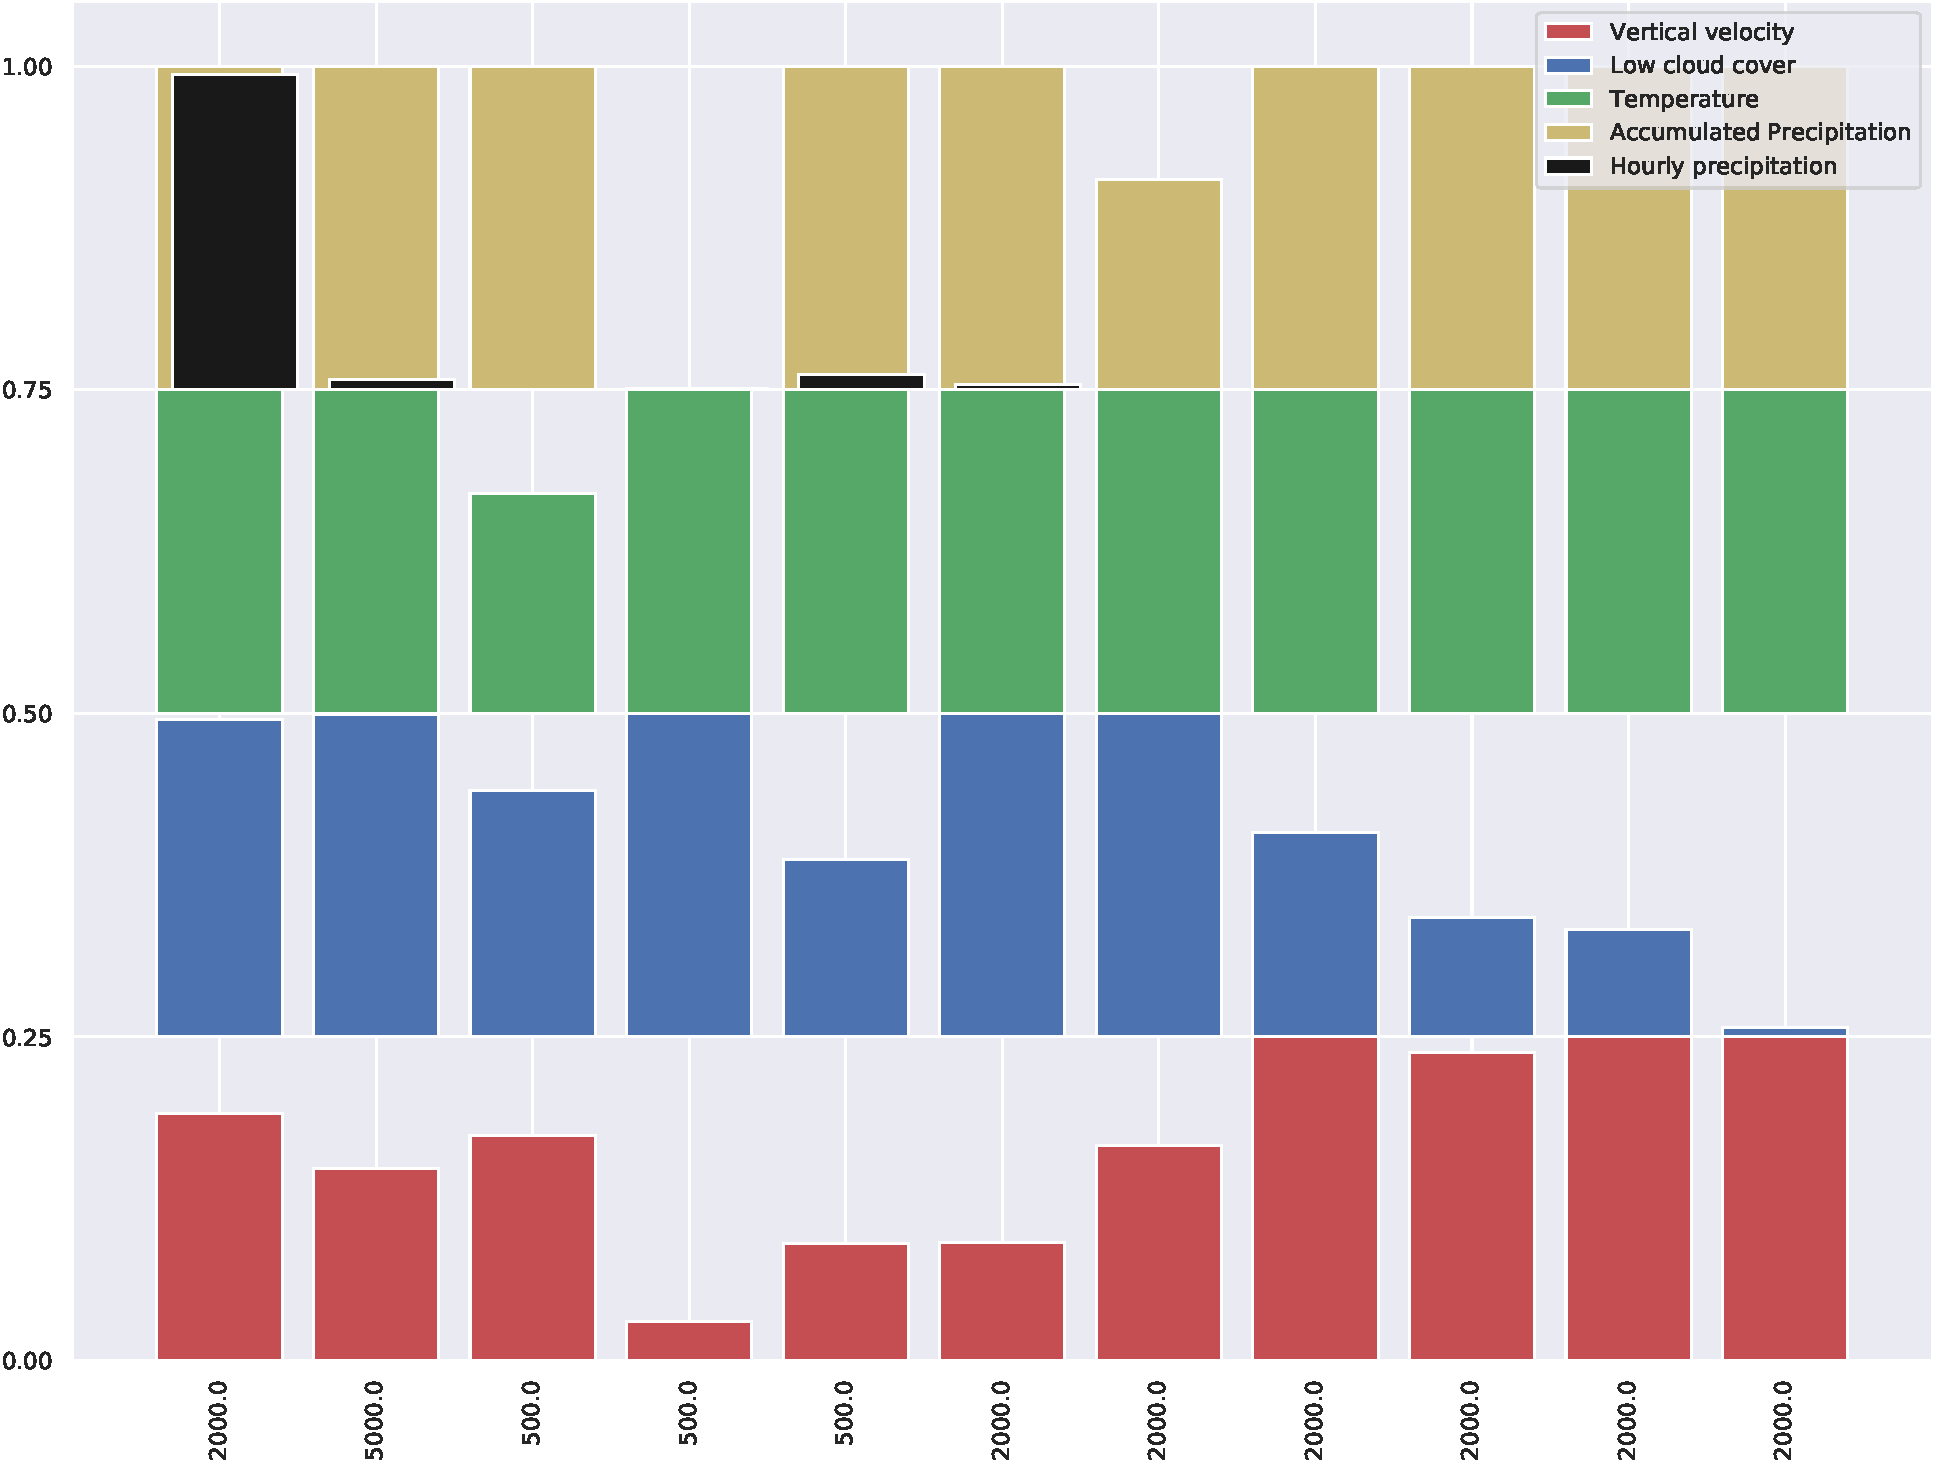
\includegraphics[width=\textwidth]{Figures/HeliDecomp.pdf}
    \caption{Same as \ref{fig:HeliAccum}, but clearly delineated between the sub-indices}
    \label{fig:HeliDecomp}
\end{figure}

\begin{figure}
    \centering
    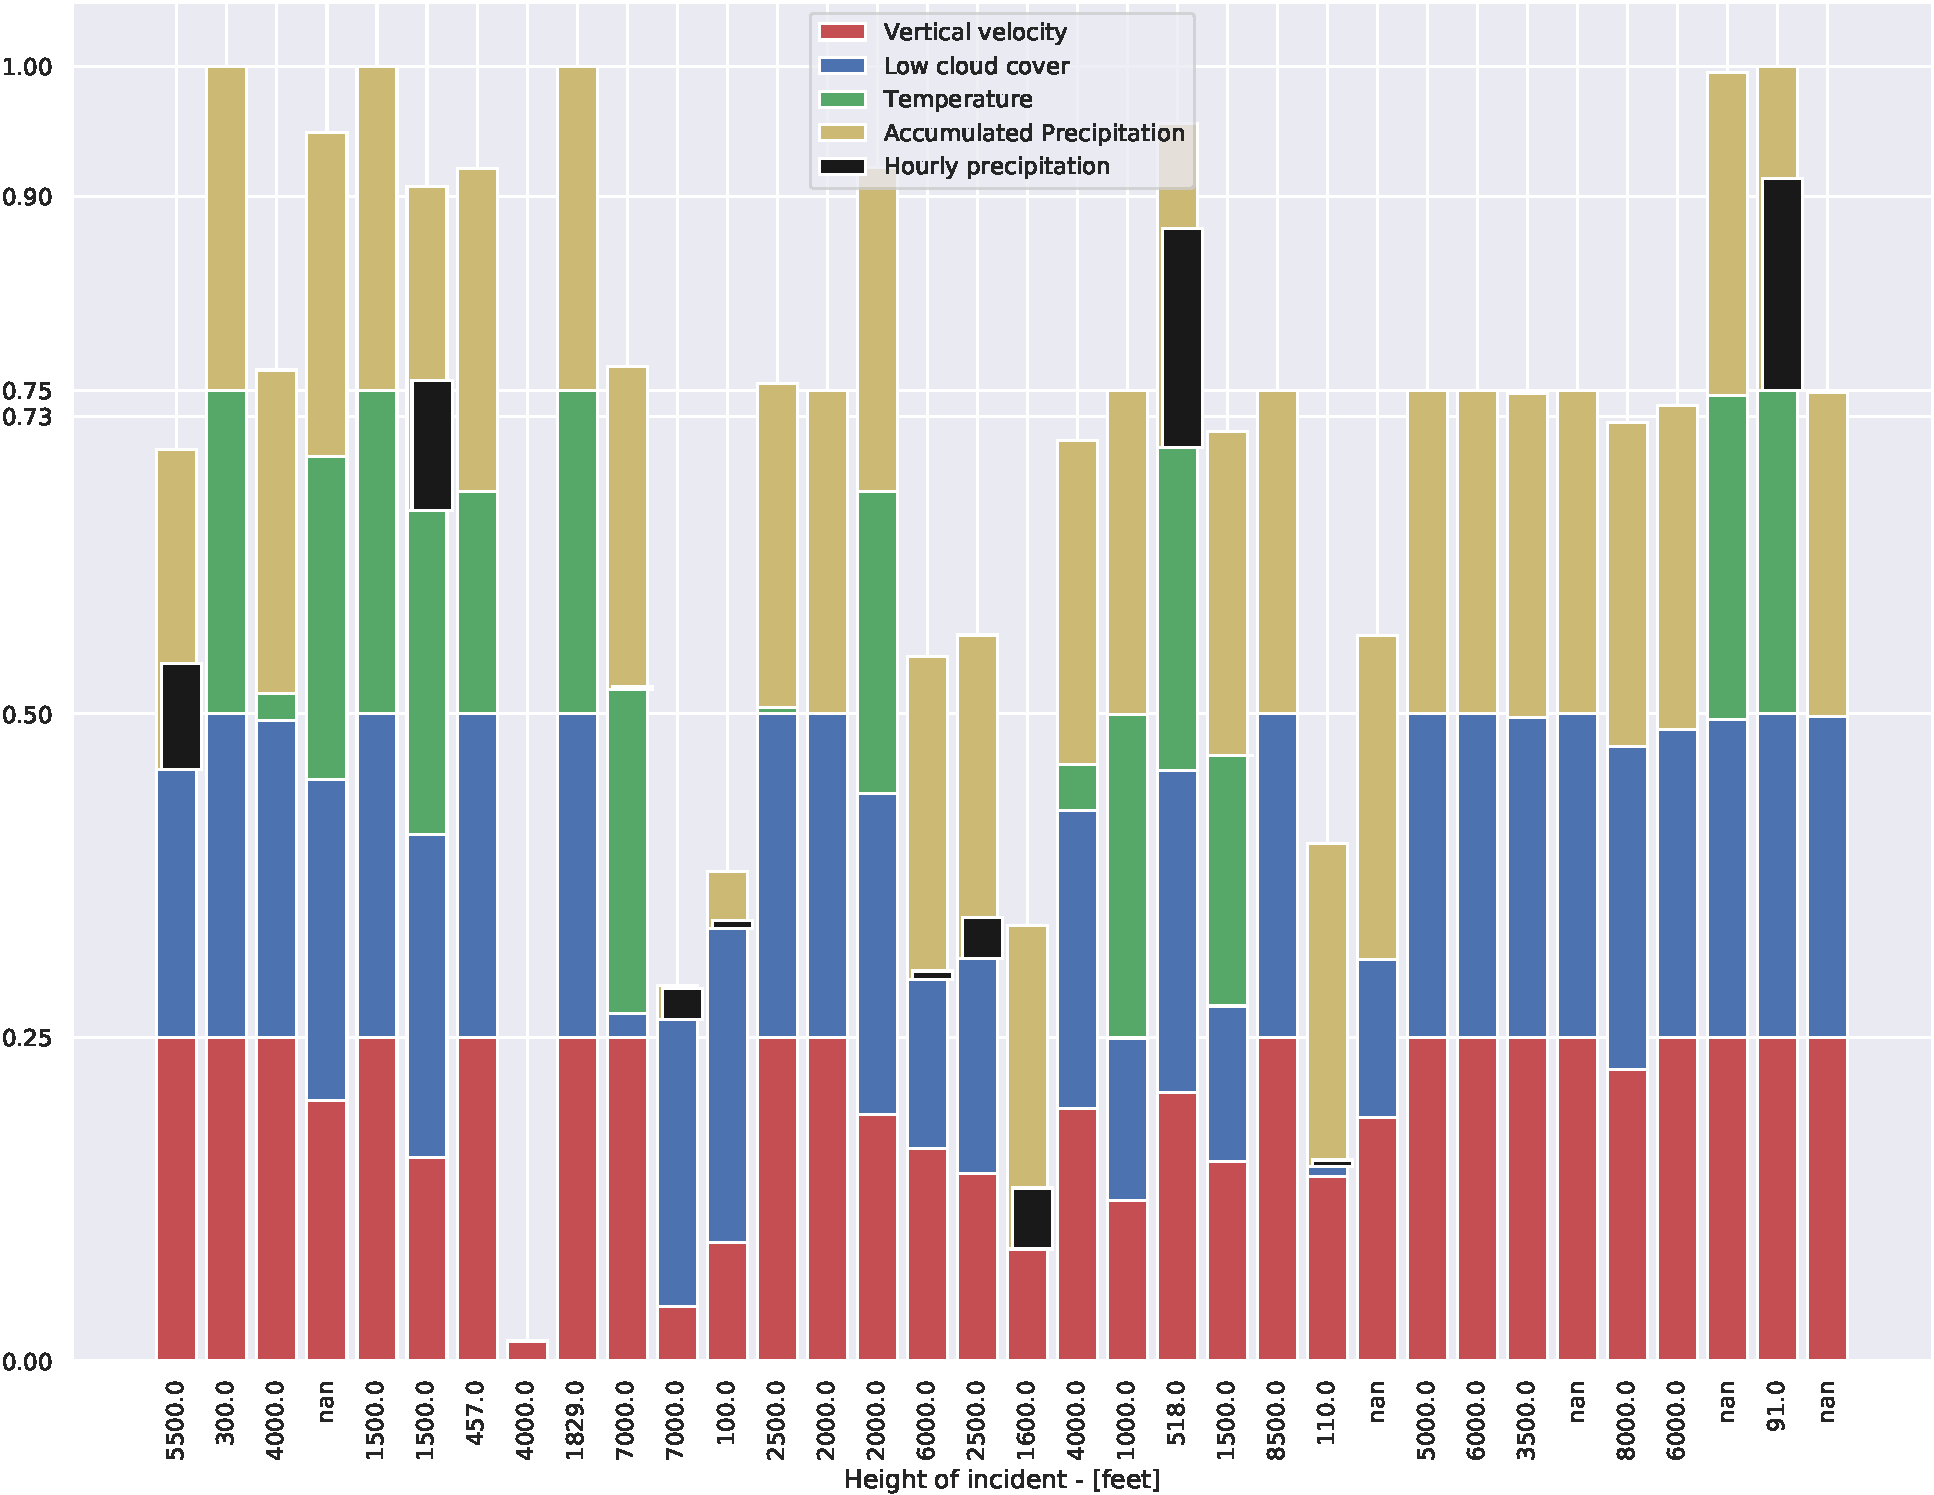
\includegraphics[width=\textwidth]{Figures/FWAccum.pdf}
    \caption{Contributions from the different sub-indices, for Fixed wing cases during the operational forecast. X-axis is height of incident in feet. Black on yellow is correction made by using the hourly precipitation instead of accumulated precipitation. Included are only cases from Avinor data set where position and height was available, for cases after November 2016.}
    \label{fig:FWAccum}
\end{figure}

\begin{table}
    \centering
    \begin{tabular}{c|c|c|c}
        Forecast & With Accumulated & Without Accumulated & Missed \\ \hline
        >Yellow (0.73) & 22 & 21 & 14 (41.2\%)\\
        >Orange (0.90) & 10& 8& 25 (73.5\%)\\ 
        >Red (0.99) & 4& 3& 30 (88.2\%)\\
    \end{tabular}
    \caption{Amount of cases forecast in each risk category based on the $34$ Fixed wing cases in Figure \ref{fig:FWAccum}. A Red risk is counted in Orange, and Yellow.}    \label{tab:FWCont}
\end{table}

\begin{figure}
    \centering
    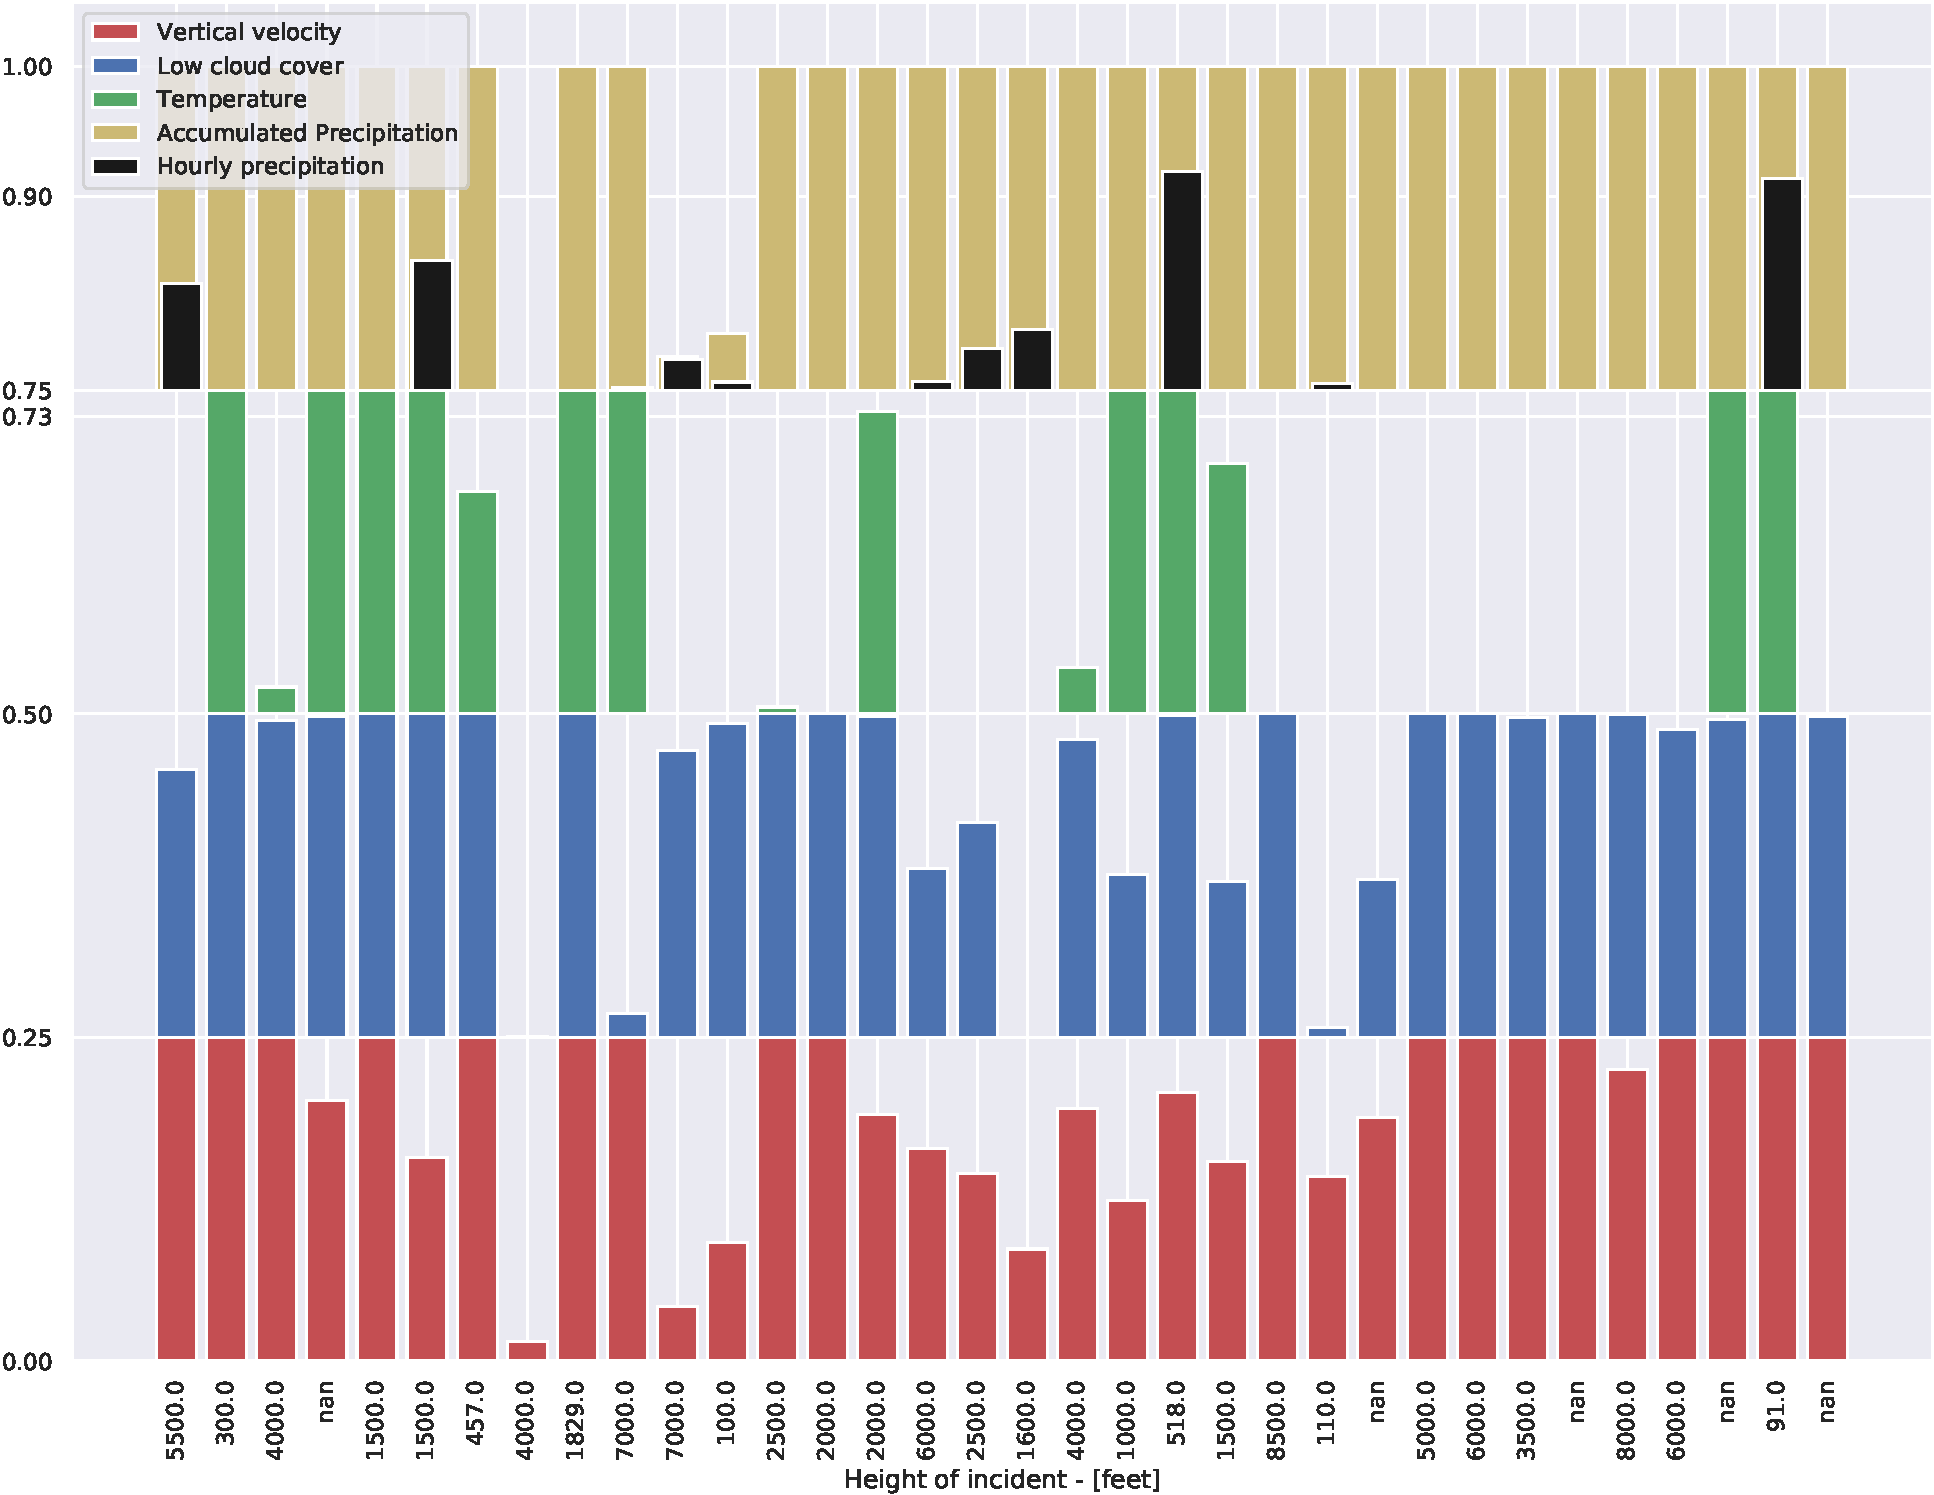
\includegraphics[width=\textwidth]{Figures/FWDecomp.pdf}
    \caption{Same as \ref{fig:FWAccum}, but clearly delineated between the sub-indices}
    \label{fig:FWDecomp}
\end{figure}
